\chapter{Automation}

Gravwell provides several utilities to enable automated operations.
At the most basic level, users can schedule searches to be executed at specific times, for
example every morning at 1:00. They can also schedule
\emph{flows} and \emph{scripts}, which can execute multiple searches, sift and parse search
results, and send notifications via email or HTTP. Flows are designed using a drag-and-drop
graphical interface and are generally preferred over scripts, which should be reserved for legacy
situations or very particular usecases which flows cannot cover.

These scheduled
operations are run by the \textbf{search agent}, a separate program which
connects to the Gravwell webserver as a client. This chapter describes
the search agent, scheduled searches, flows, and scripts.

\section{Configuring User Email Settings}

In order to send emails from scheduled scripts, each user must input
settings for their preferred email server. This will allow Gravwell to
act as an SMTP client and send emails on the user's behalf. The email
configuration page is a sub-tab in the user's account settings (see Figure \ref{fig:email-prefs}).

\begin{figure}
	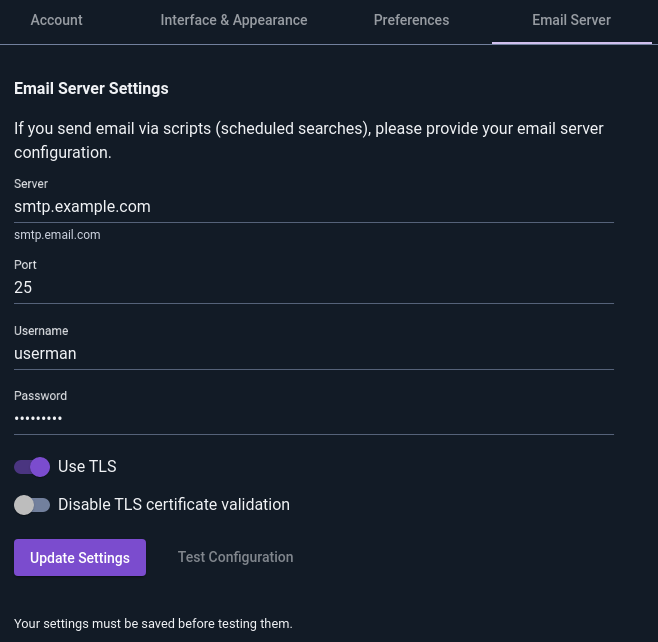
\includegraphics[width=0.7\linewidth]{images/email-prefs.png}
	\caption{Email preferences dialog}
	\label{fig:email-prefs}
\end{figure}

The Username and Password fields should be filled out with the user's
authentication tokens for the \emph{email server}. If TLS is required by
the server, set the `Use TLS' toggle; note that it may be necessary to
change the Port to 465 after enabling TLS.

After populating the configuration, hit `Update Settings' to save the
options. `Test Configuration' should then become clickable. Click it to
bring up the email testing
dialog, as seen in Figure \ref{fig:email-testing}.

\begin{figure}
	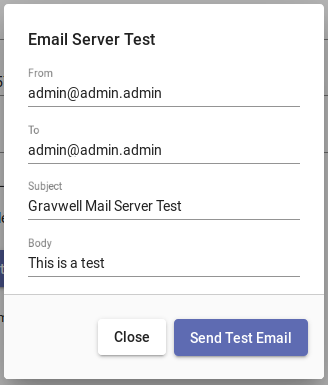
\includegraphics[width=0.5\linewidth]{images/email-testing.png}
	\caption{Email testing dialog}
	\label{fig:email-testing}
\end{figure}

Change the ``From'' and ``To'' addresses to the user's own email
address, then click `Send Test Email'. Gravwell will attempt to use the
mail server to send an email to the user. If the email arrives, the
email server has been correctly configured. It may be necessary to check
spam folders.

If the email does not arrive, check the Gravwell webserver logs,
located in \code{/opt/gravwell/log/web} by default.


\section{The Search Agent}

The search agent is the Gravwell component which actually handles the
execution of scheduled searches and scripts. It is a separate process
which connects to a Gravwell webserver as a client, obtains a list of
scheduled searches/scripts, and runs them when scheduled.

The search agent is shipped in the main Gravwell installer and should
be installed by default in most situations. If for some reason the
search agent is not enabled, a notification will appear in the Gravwell
web interface warning of that fact (Figure \ref{fig:searchagent-warn}).

\begin{figure}
	
\includegraphics[width=0.4\linewidth]{images/searchagent-warn.png}
	\caption{Search agent warning}
	\label{fig:searchagent-warn}
\end{figure}

Note that when using multiple Gravwell webservers, the search agent
should be disabled on all but one of them to avoid conflicts and
superfluous search executions.

\subsection{Disabling the Search Agent}

To disable the search agent on a server that uses Systemd:

\begin{Verbatim}[breaklines=true]
systemctl stop gravwell_searchagent.service
systemctl disable gravwell_searchagent.service
\end{Verbatim}

The Docker images provided by Gravwell do not use Systemd; instead,
they use a Gravwell-implemented process manager called ``manager''\footnote{https://github.com/gravwell/manager}. To disable the search agent on such a
container, pass the argument \code{-e DISABLE\_SEARCHAGENT=TRUE} when
creating the container, e.g.:

\begin{Verbatim}[breaklines=true]
docker run --rm --net gravnet -p 8080:80 -d \
-e DISABLE_SEARCHAGENT=TRUE --name gravwell gravwell:base
\end{Verbatim}

\subsection{Search Agent Configuration}

Although the search agent ships with the indexer and webserver
components, it uses its own configuration file found at
\code{/opt/gravwell/etc/searchagent.conf}. While the defaults set at
install time should be sufficient, this section describes the
configuration options in case changes are needed.

\subsubsection{Webserver-Address}

The \code{Webserver-Address} parameter should be an IP or hostname and a
port which point to the Gravwell webserver. If no port is specified,
port 443 is used by default (80 if HTTPS is disabled). The following are
all valid Webserver-Address values:

\begin{Verbatim}[breaklines=true]
Webserver-Address=10.0.0.1:80
Webserver-Address=127.0.0.1:443
Webserver-Address=192.168.0.1
Webserver-Address=gravwell-webserver.example.com
\end{Verbatim}

If Webserver-Address is specified multiple times, the search agent will multiplex
scheduled searches across all listed servers, to distribute load.

\subsubsection{Search-Agent-Auth}

The \code{Search-Agent-Auth} parameter specifies the token which is used to
authenticate with the webserver. This can be any string, but it
\emph{must} correspond with the \code{Search-Agent-Auth} parameter defined in
the webserver's \code{gravwell.conf}!

\subsubsection{Insecure-Use-HTTP}

Setting the \code{Insecure-Use-HTTP} parameter to ``true'' instructs the
search agent to connect to the Gravwell webserver using unencrypted
HTTP. This should only be used on trusted internal networks or on the
local loopback interface!

\subsubsection{Insecure-Skip-TLS-Verify}

Setting the \code{Insecure-Skip-TLS-Verify} parameter to true instructs
the search agent to ignore invalid TLS certificates when connecting to
the webserver.

\subsubsection{Log-File}

\code{Log-File} specifies a file where the search agent should write its
logs. If not set, the search agent will write logs to standard error.

\subsubsection{Log-Level}

\code{Log-Level} sets the severity level at which log entries will actually be
written to the log, thus setting \code{Log-Level=WARN} ensures only warnings,
errors, and critical messages will be sent to the log. The available
levels are OFF, DEBUG, INFO, WARN, ERROR, and CRITICAL.

\subsubsection{Max-Script-Run-Time}

The \code{Max-Script-Run-Time} parameter specifies how long, in minutes, a
given scheduled script is allowed to execute. If set to 0, scripts can
run for an unlimited length of time. There are two things to consider
when setting this:

\begin{enumerate}
\tightlist
\item
  A script which runs indefinitely only interferes with itself; other
  scheduled searches and scripts will run regardless.
\item
  Many buggy scripts will automatically time out, because a script must
  also execute at least one of the Gravwell-defined
  scripting functions every 30 seconds. A hung script will quickly
  be terminated.
\end{enumerate}


\subsection{Scheduling Searches}

Users can schedule searches to run at regular intervals. This enables
several useful possibilities, such as automatically updating lookup
tables (e.g. MAC address to IP mappings) or executing a very detailed /
long-running search every morning at 6 a.m. to have the results ready
when employees arrive.

\subsubsection{Creating a Scheduled Search}

To create a scheduled search, select the `Scheduled Searches' page from
the menu in the GUI, then click the `Add' button in the upper right
corner of the page. A form will pop up, as shown in Figure \ref{fig:new-scheduled}.

\begin{figure}
	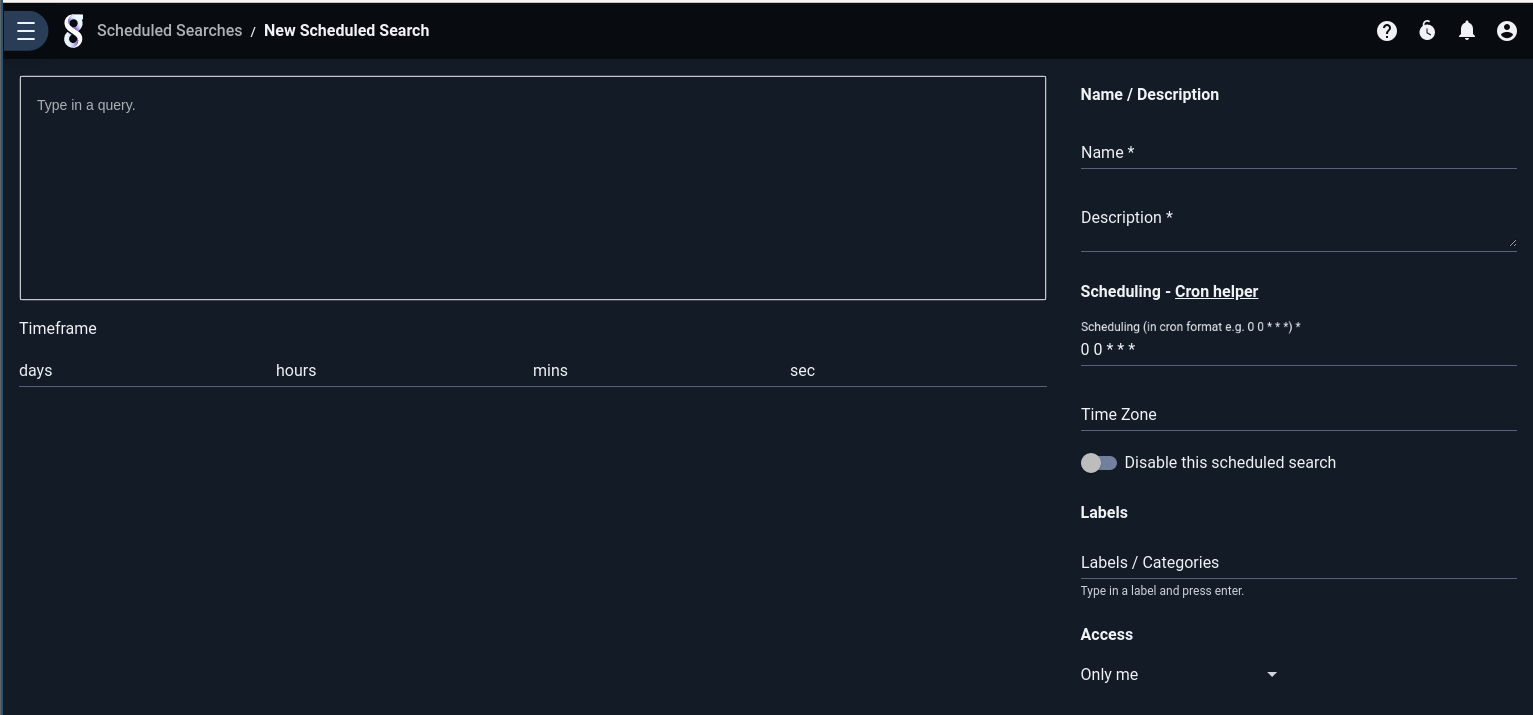
\includegraphics{images/new-scheduled.png}
	\caption{New scheduled search form}
	\label{fig:new-scheduled}
\end{figure}

Enter the desired query in the box labeled `Type in a query', then use
the timeframe picker to choose how far back the search should run.
Assign the scheduled search a name and a description.

The `Scheduling' field requires some explanation. This field defines a
cron-formatted schedule to specify when the search should run. Clicking
the `Cron Helper' link will open a useful website to experiment with
cron schedules. The following are all valid schedules:

\begin{itemize}
\tightlist
\item
  Run every minute: \code{* * * * *}
\item
  Run every 10 minutes: \code{*/10 * * * *}
\item
  Run every hour: \code{0 * * * *}
\item
  Run every day at 2 a.m.: \code{0 2 * * *}
\item
  Run once a week at 7 P.M.: \code{0 19 */7 * *}
\end{itemize}

When all the fields have been populated, click `Save' to save the
scheduled search. The search agent will soon discover this new search
and will execute it on schedule.

\subsubsection{Viewing Scheduled Search Results}

Once a scheduled search has been executed at least once, the results of
the most recent search execution are available for review. Although the
search results appear in the `Persistent Searches' page, the simplest
way to view the results for a particular scheduled search is to select
the `Run last search' icon on the tile for that scheduled search within
the `Scheduled Searches' page (Figure \ref{fig:run-last-search}).

\begin{figure}
	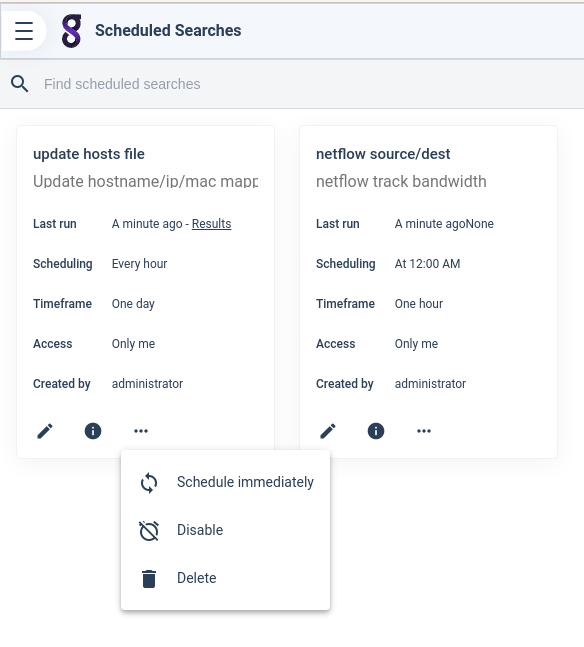
\includegraphics{images/run-last-search.png}
	\caption{The ``Run last search'' button}
	\label{fig:run-last-search}
\end{figure}

This will open the most recent results from that scheduled search. Note
that when the search agent runs a scheduled search, it deletes the
previous run's results when the new search completes. This prevents old
searches from cluttering the disk.

\subsection{Hands-On Lab}

This lab will demonstrate how a scheduled search can automatically
update lookup tables. First, create a Gravwell webserver+indexer
container:

\begin{Verbatim}[breaklines=true]
docker run -d --rm --net gravnet -p 8080:80 --name gravwell gravwell:base
\end{Verbatim}

Then we'll use the ingesters container (make sure you've loaded the ingesters container image as described in Section \ref{sec:load-lab-images}) to import some DHCP data:

\begin{Verbatim}[breaklines=true]
cd ~/gravwell_training/Automation/Lab-Scheduled

docker run -v $PWD/data:/tmp/data --rm -i --net gravnet \
gravwell:ingesters /opt/gravwell/bin/reimport -rebase-timestamp \
-clear-conns gravwell:4023 -i /tmp/data/dhcp.json.gz -import-format json \
-tag-override syslog
\end{Verbatim}

Log into the web GUI (\href{http://localhost:8080}{http://localhost:8080}).
 A simple search on the ``syslog'' tag over the last two weeks should show some results
similar to Figure \ref{fig:dhcp-data}.

\begin{figure}
	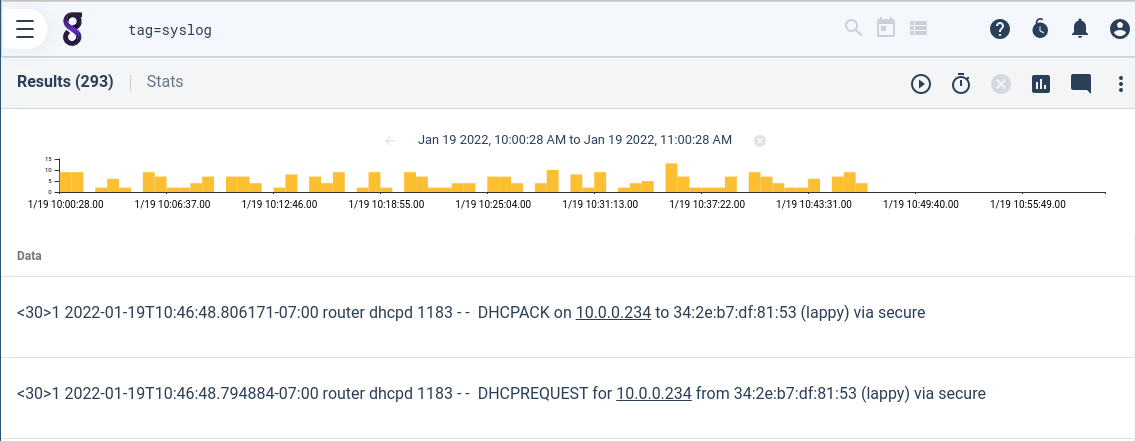
\includegraphics{images/dhcp-data.png}
	\caption{Raw DHPC logs}
	\label{fig:dhcp-data}
\end{figure}

These DHCP server logs can be used by a scheduled search to build a
lookup table for search enrichment, mapping MAC addresses and IP
addresses to hostnames. Go to the Scheduled Searches page, click `Add',
and fill in the form with the following:

\begin{itemize}
\item
  \textbf{Query:} 
\begin{Verbatim}[breaklines=true]
tag=syslog regex "HOSTNAME: (?P<hostname>\S+) on (?P<ip>\S+) at (?P<mac>\S+)" 
| unique hostname ip mac 
| table -save hosts hostname ip mac
\end{Verbatim}
\item
  \textbf{Timeframe:} \code{14 days}
\item
  \textbf{Name:} \code{hostsfile}
\item
  \textbf{Description:} \code{update hosts file}
\item
  \textbf{Scheduling:} \code{~* * * * *}
\end{itemize}

This scheduled search will run every minute, searching over the last 14
days to extract MAC:IP:hostname mappings. It will use the table
renderer's \code{-save} flag to save the results in a resource named
``hosts''.

Within a minute, a resource named ``hosts'' should appear on the
Resources page. We will test this lookup table by attempting to look up
the hostname which corresponds to the IP requested in DHCPREQUEST
messages. Here is a sample DHCPREQUEST message:

\code{\textless{}190\textgreater{} 11:15:02 apu dhcpd: DHCPREQUEST for
192.168.2.52 from 08:00:27:ca:b2:e7 via igb2}

From this, we can create a regular expression which extracts the IP
address, then use the new lookup table to match that IP address against
a hostname in the hosts resource. Figure \ref{fig:lookup-results} shows the
results.

\begin{Verbatim}[breaklines=true]
tag=syslog regex "DHCPREQUEST for (?P<ip>\S+)" 
| lookup -r hosts ip ip hostname as hostname | table
\end{Verbatim}

\begin{figure}
	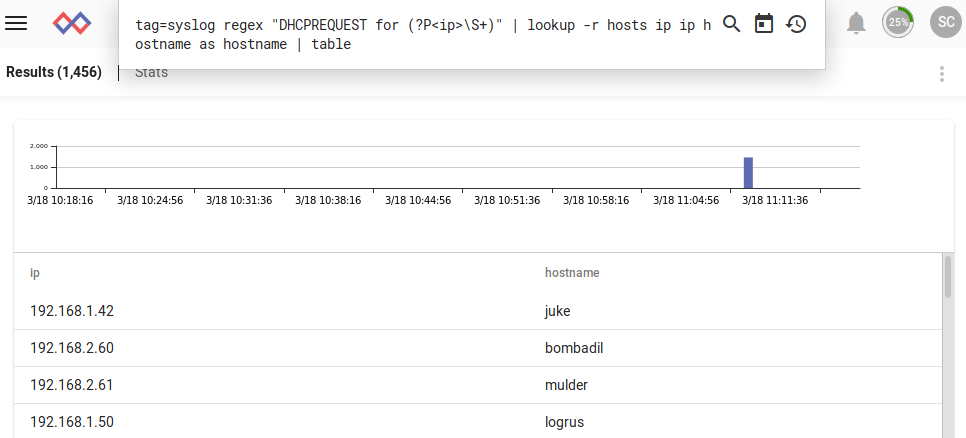
\includegraphics{images/lookup-results.png}
	\caption{Lookup table results}
	\label{fig:lookup-results}
\end{figure}

To clean up after the experiment, simply run:

\code{docker kill \$(docker ps -a -q)}

%%%%%%%%%%%%%%%%%%%%%%%%%%%%%%%%%%%%%%%%%%%%%%%%%%
% FLOWS
%%%%%%%%%%%%%%%%%%%%%%%%%%%%%%%%%%%%%%%%%%%%%%%%%%
\section{Flows}
\index{Automation!flows|see {Flows}}\index{Flows}
Flows provide a no-code method for developing advanced automations in Gravwell. A flow consists of one of more \emph{nodes}; each node performs a single action and passes the results (if any) on to the next node(s). By wiring together nodes in a drag-and-drop user interface, users can:

\begin{itemize}
\tightlist
\item Run queries
\item Generate PDF reports
\item Send emails
\item Fire off Slack and MS Teams messages
\item Re-ingest alerts
\item etc.
\end{itemize}

\subsection{Flow Concepts}
\label{sec:flow-concepts}

Flows are automations, meaning they are normally executed on a user-specified schedule by the search agent. They can also be run manually through the user interface. The basic process of flow development is:

\begin{enumerate}
\item Create a new flow
\item Instantiate nodes in the flow and connect them together
\item Configure nodes
\item Test the flow with debug runs
\item Deploy the flow by setting a schedule \& enabling scheduled execution
\end{enumerate}

\subsubsection{Nodes}
\index{Flows!nodes}
A flow is a collection of \emph{nodes}, linked together to define an order of execution. Each node does a single task, such as running a query or sending an email. Figure \ref{fig:nodes} shows a simple flow of three nodes; the leftmost node runs a Gravwell query, then the middle node formats the results of that query into a PDF document, and finally the rightmost node sends that PDF document as an email attachment.

\begin{figure}
	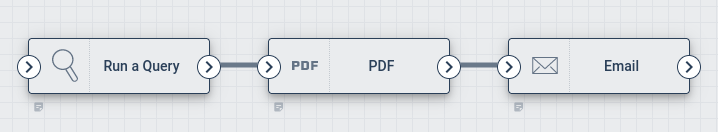
\includegraphics[width=0.7\linewidth]{images/nodes.png}
	\caption{A simple flow with three nodes.}
	\label{fig:nodes}
\end{figure}

All nodes have a single output socket. Most have only a single input socket, but some nodes which merge \emph{payloads} (see below) have multiple input sockets. One node's output socket may be connected to the \emph{inputs} of multiple other nodes, but each input socket can only take one connection.

\subsubsection{Payloads}
\index{Flows!payloads}
\emph{Payloads} are collections of data passed from node to node, representing the state of execution. For instance, the ``Run a Query'' node will insert an item named ``search'' into the payload, containing things like the query results and metadata about the search. The PDF node can \emph{read} that ``search'' item, format it into a nice PDF document, and insert the PDF file back into the payload with a name like ``gravwell.pdf''. Then the Email node can be configured to attach ``gravwell.pdf'' to the outgoing email.

Most nodes receive a single incoming payload through a single \emph{input} socket, then pass a single outgoing payload via the \emph{output} socket. In most cases, the outgoing payload will be a modified version of the incoming payload.

The \emph{merge} nodes are exceptions to this general rule. The Stack Merge and Nest Merge nodes take multiple incoming payloads (via multiple input sockets) and merge them into a single output. See Section \ref{sec:nodes} for more detailed descriptions of these nodes.

\subsubsection{Execution order}

Nodes are always executed one at a time. A node can be executed if all nodes upstream of it (its \emph{dependencies}) have executed. If multiple nodes are ready to execute, one will be chosen at random. In Figure \ref{fig:execution}, both the ``Run a Query'' node and the ``HTTP'' node are candidates to run first. After the Query node finishes, the If node can execute; when it is done, the Slack Message node may run. We say that the ``If'' node is \emph{downstream} of the Query node, and the Slack node is \emph{downstream} of both the If and Query nodes.

\begin{figure}
	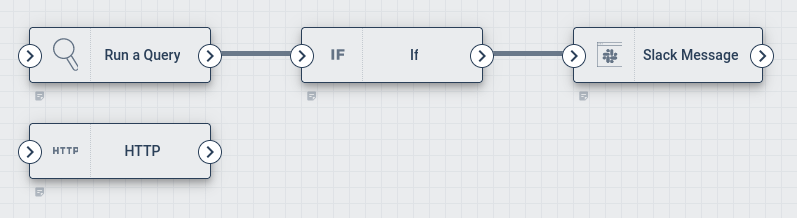
\includegraphics[width=0.7\linewidth]{images/execution.png}
	\caption{An illustration of execution order.}
	\label{fig:execution}
\end{figure}

Note that some nodes may block execution of downstream nodes. The \code{If} node is configured with a boolean logic expression; if that expression evaluates to \emph{false}, none of the If node's downstream nodes are executed. Nodes which can block downstream execution will always have a note to that effect in the online documentation.

\subsection{The Flow Editor}
\index{GUI!flow editor}
Flows are created using the flow editor. Although the Gravwell flow editor can be intimidating at first glance, a few minutes' worth of experimentation and exploration should be enough to get started building flows. This section will go through the various components of the UI, explaining each component.

Note: If you're not yet familiar with the basic components of a flow (nodes, sockets, payloads), refer to Section \ref{sec:flow-concepts} for an overview.

You can access the flow editor from the Query \& Dev Studio interface, found in the Main Menu. Select ``Flows'' from the left-hand side, as shown in Figure \ref{fig:dev-studio-newflow}. From there, you can either start a new blank flow (``Start a New Flow'') or instantiate one of the ``starter flows'' provided by Gravwell.

\begin{figure}
	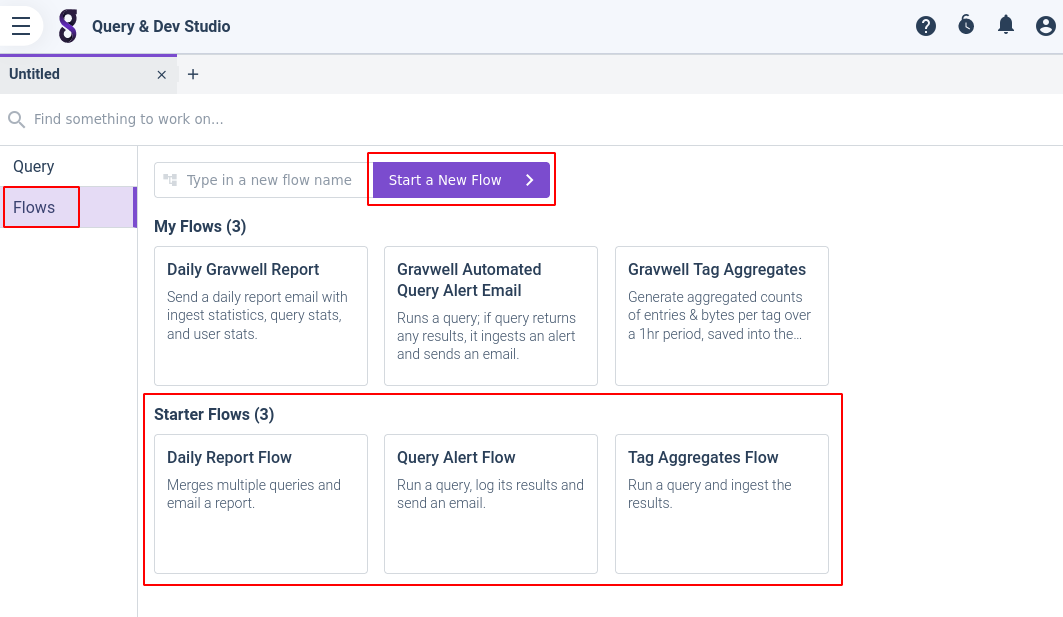
\includegraphics[width=0.8\linewidth]{images/dev-studio-newflow.png}
	\caption{Flows in the Query Studio}
	\label{fig:dev-studio-newflow}
\end{figure}

Selecting either option will take you into the flow editor, the parts of which are marked in Figure \ref{fig:flow-editor}. The \emph{palette} provides a list of available nodes, which can be dragged out into the \emph{canvas}. The \emph{console} provides information about problems with the flow and output from any test runs.

\begin{figure}
	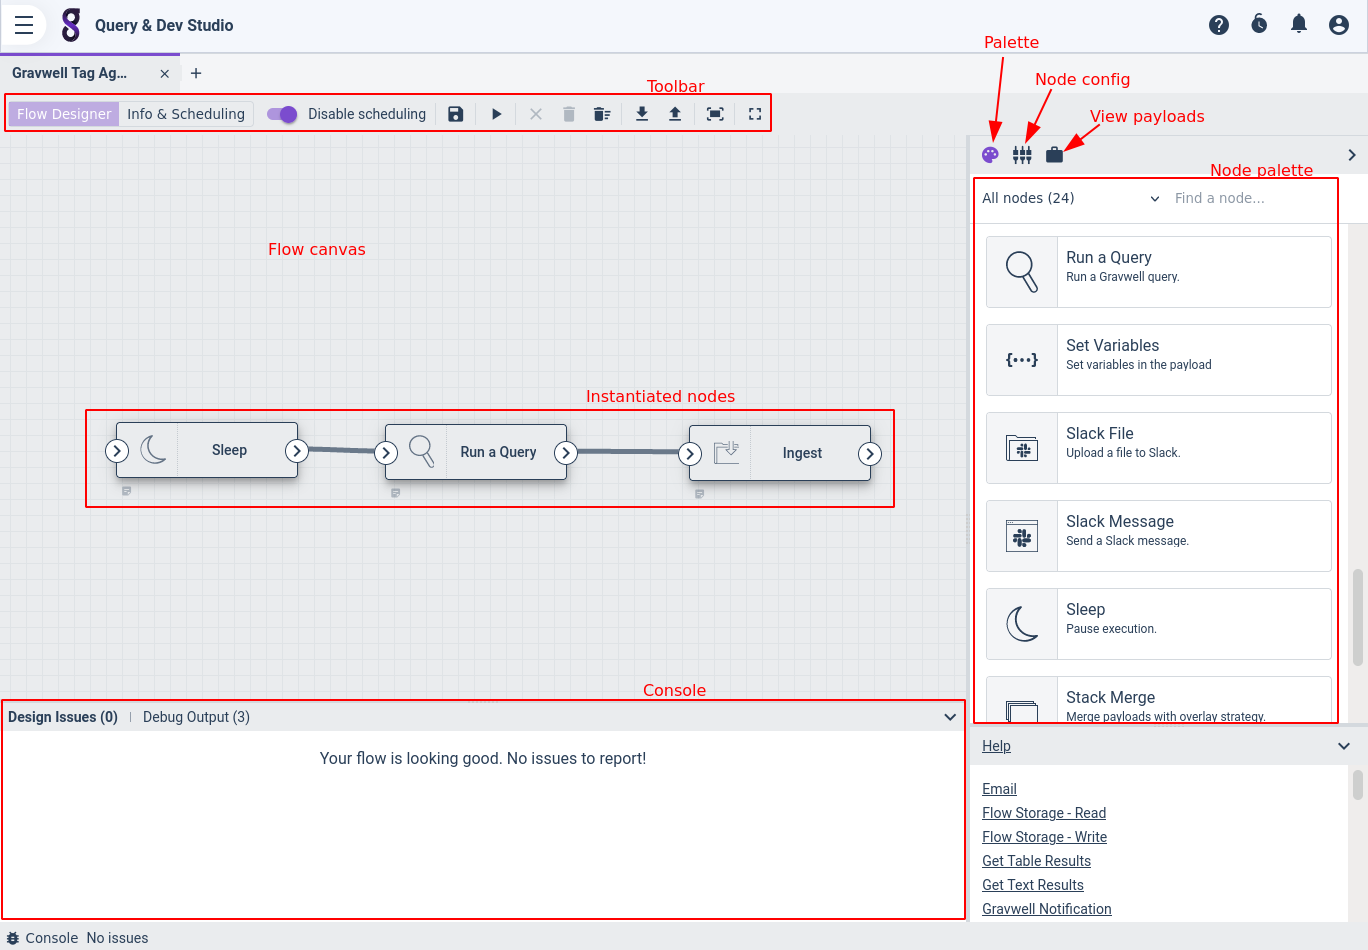
\includegraphics[width=0.85\linewidth]{images/flow-editor.png}
	\caption{Parts of the Flow Editor.}
	\label{fig:flow-editor}
\end{figure}

Nodes are instantiated by dragging them from the palette onto the canvas. Once on the canvas, node input and output sockets can be connected, nodes can be re-arranged, etc. Note that the scroll wheel can be used to zoom in and out of the canvas view.

The toolbar contains buttons for quick access to editor functionality. From left to right:

\begin{itemize}
\item Flow Designer: shows the flow canvas (default view).
\item Info \& Scheduling: shows options to set flow name, description, scheduling, sharing, etc.
\item Disable scheduling: toggle to quickly enable/disable automatic execution of the flow.
\item Save: save the flow.
\item Debug: run the flow
\item Clear selection: deselects any currently-selected node.
\item Delete: delete the selected node.
\item Delete all: delete all nodes (requires confirmation).
\item Export flow: download the flow specification, for backup or sharing.
\item Import flow: upload a previously-exported flow spec.
\item Fit all nodes on screen: zoom \& center the canvas so that \emph{all} nodes are visible.
\item Fullscreen: puts the editor into fullscreen mode.
\end{itemize}

\subsubsection{Configuring Nodes}

Once a node has been instantiated by dragging it from the palette to the canvas, it must be configured. Clicking on the node will bring up the configuration pane as seen in Figure \ref{fig:node-config}.

\begin{figure}
	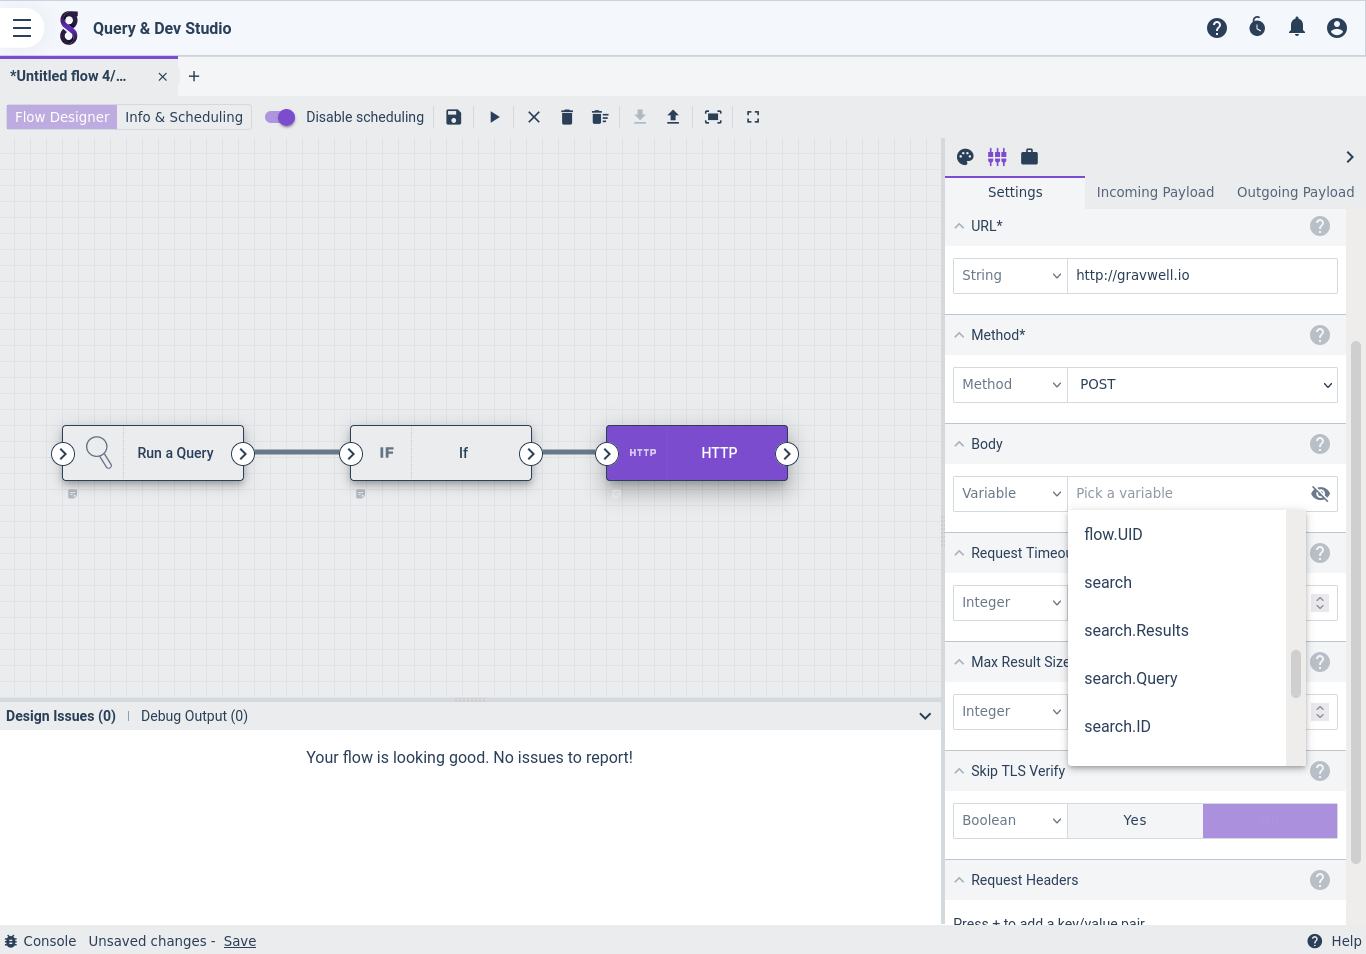
\includegraphics[width=0.85\linewidth]{images/node-config.png}
	\caption{Configuring a node.}
	\label{fig:node-config}
\end{figure}

The HTTP node shown in Figure \ref{fig:node-config} is a particularly complex node with many config options, which serves well for demonstration. Note that the URL and Method fields are marked with an asterisk, indicating that they are required. Note also the drop-down menus for each config option; these allow you to change between entering a constant value (e.g. the string ``http://gravwell.io'' in the URL config) or selecting a value from the payload as shown with the Body config.


If a node is misconfigured, the console will display a list of problems. In Figure \ref{fig:parse-errors}, we see that the Email node has several config options which are not yet set. As those options are populated, the errors will go away.

\begin{figure}
	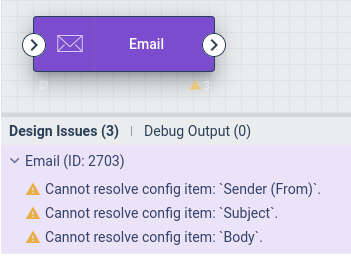
\includegraphics[width=0.85\linewidth]{images/parse-errors.png}
	\caption{Parse errors.}
	\label{fig:parse-errors}
\end{figure}

Note: You can return to the palette view at any time by clicking the palette icon above the configuration pane.

\subsubsection{Debugging}

Once a flow has been designed and configured, it can be debugged. This will signal the search agent component that it should try executing the flow. To start a debug run, click the ``Run flow and debug'' button (the ``play button'') in the toolbar. The user interface will then wait for the search agent to complete its run.

Once the run is complete, the console will have detailed execution information for each node in the ``Debug Output'' pane. The nodes are listed in order of execution. Clicking on a node in the debug output will bring up a pane showing that node's log output and the actual contents of that node's output payload. In Figure \ref{fig:if-payload}, we can see that the If node received a payload where \code{search.Count} was ``10'', meaning the If node's boolean statement evaluated to true and the HTTP node was allowed to execute:

\begin{figure}
	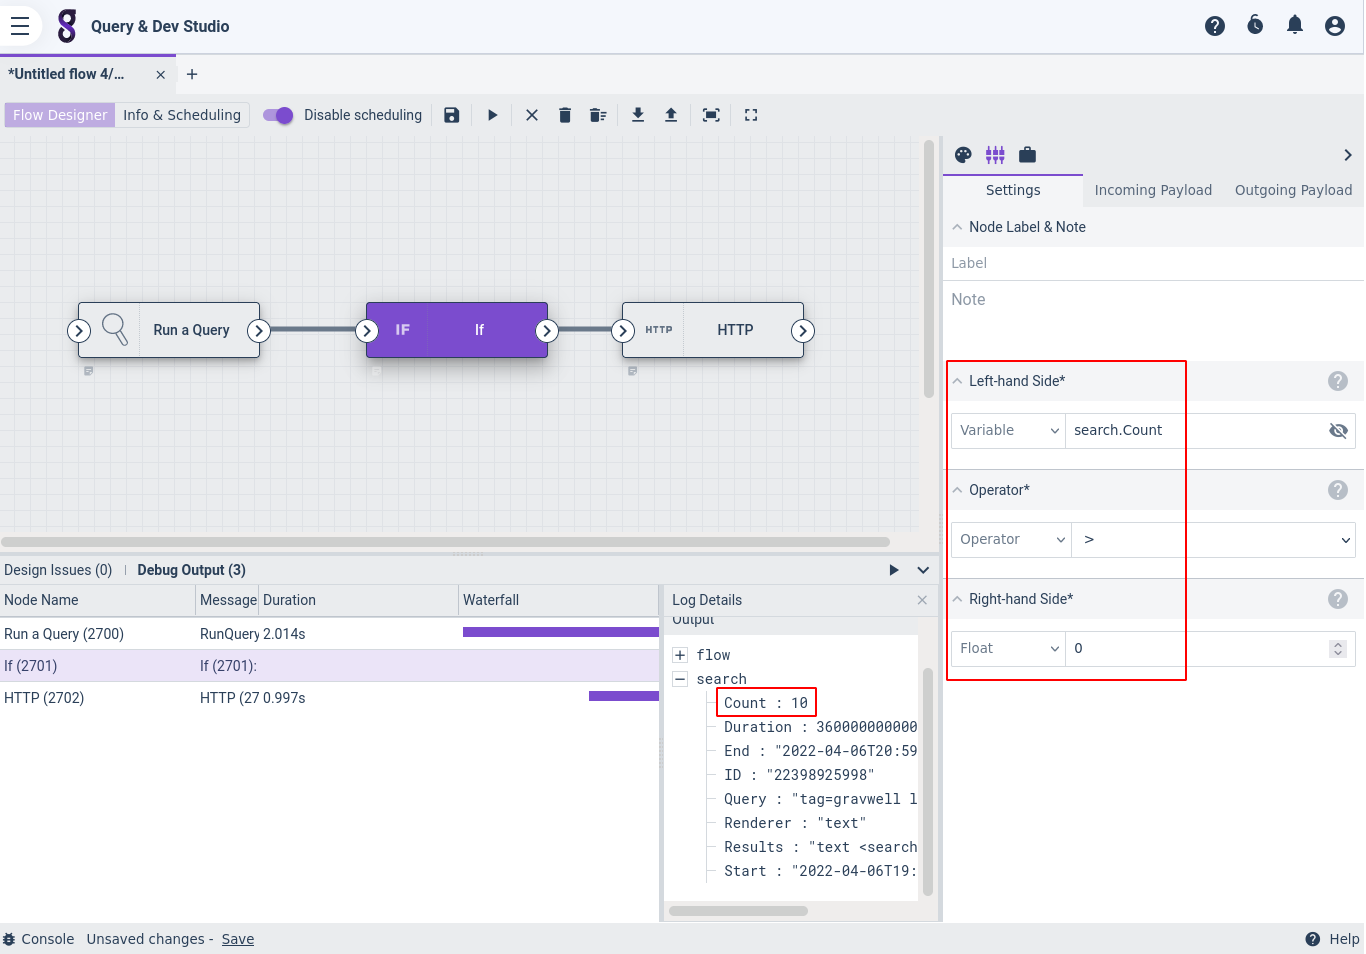
\includegraphics[width=0.85\linewidth]{images/if-payload.png}
	\caption{Node payload showing If node payload.}
	\label{fig:if-payload}
\end{figure}

If we modify the If node's config so the statement is \code{search.Count <= 0} and re-run the flow, we'll see that it now evaluates to false and the HTTP node does not execute (as seen by the empty ``Message'' column in the Debug Output pane), as shown in Figure \ref{fig:if-false}

\begin{figure}
	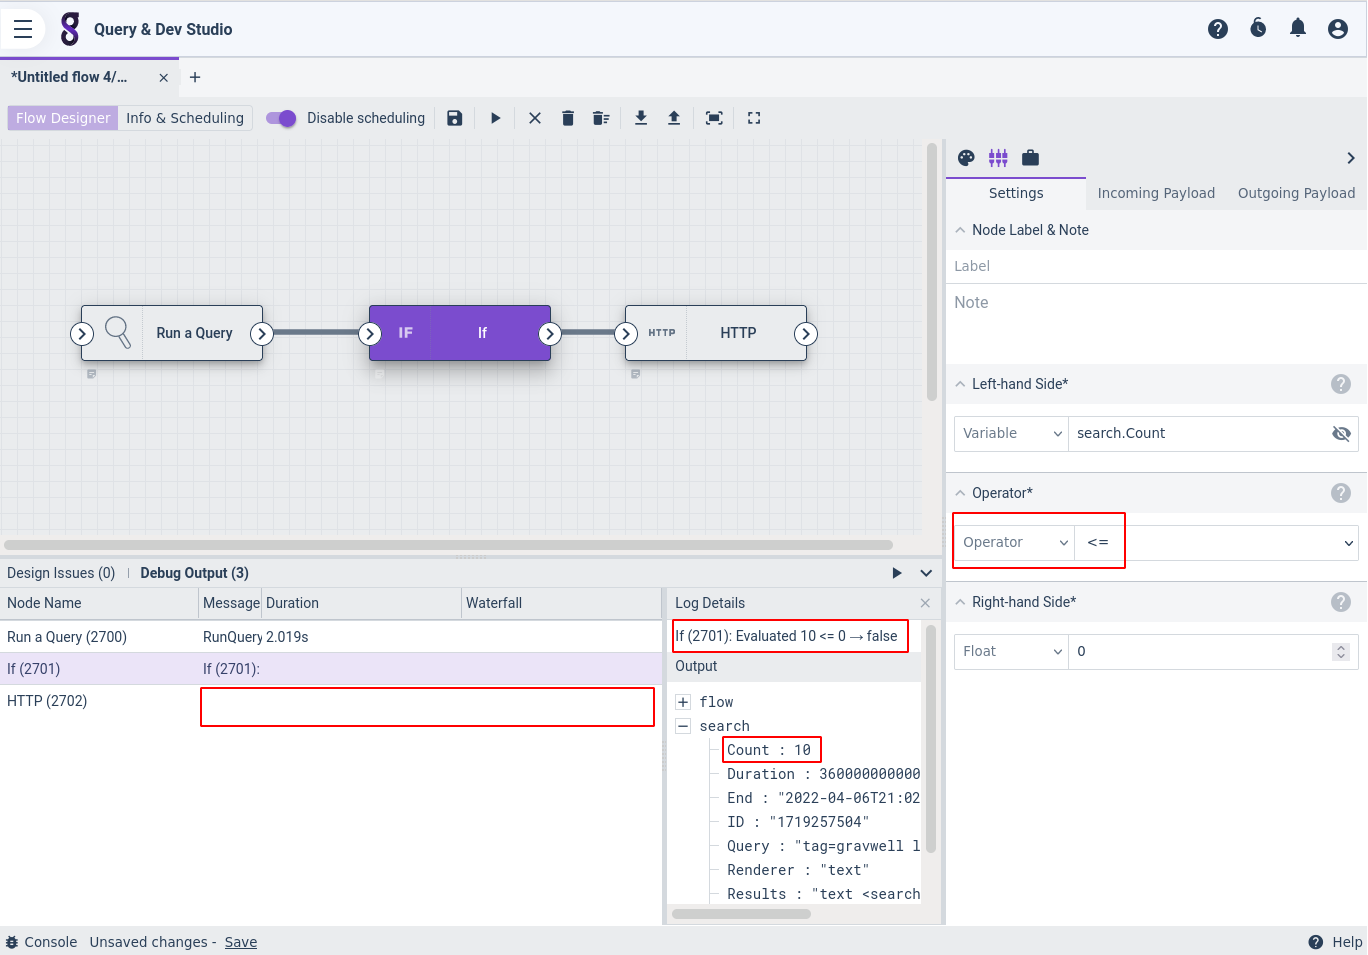
\includegraphics[width=0.85\linewidth]{images/if-false.png}
	\caption{Debug run where If node evaluates to false and execution halts.}
	\label{fig:if-false}
\end{figure}

\subsubsection{Info \& Scheduling}

Once you're happy with a flow, the final step is to give it a schedule and enable it. This is done in the ``Info \& Scheduling'' page, accessible via a button in the toolbar.

You should specify a name and description for the flow, then define a schedule. The schedule is set in cron format\footnote{https://cron.help/}, which is very flexible but can also be intimidating. There are a few shortcuts for simple cases: \code{@hourly} runs at the start of every hour, \code{@daily} at midnight every day, and so on.

\begin{figure}
	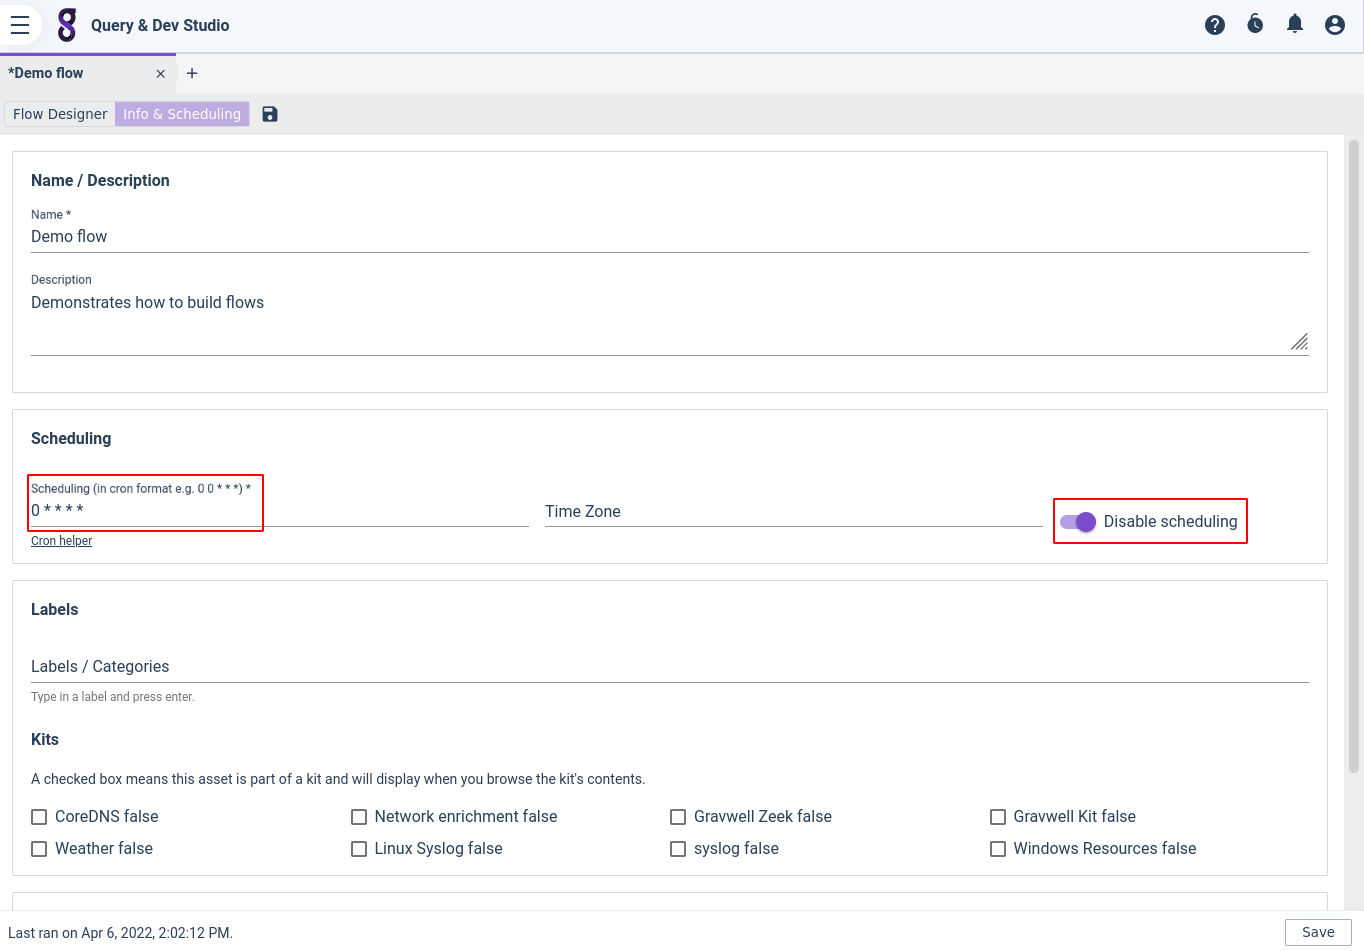
\includegraphics[width=0.85\linewidth]{images/scheduling.png}
	\caption{Info \& scheduling page for flows.}
	\label{fig:scheduling}
\end{figure}

Once the schedule is set, toggle the ``Disable scheduling'' option to enable scheduled executions of the flow. The search agent will then automatically run it on the given schedule.

\subsubsection{In-Flow ``Sticky'' Notes}

The ``Note'' node is a special node used to annotate flows. Unlike other nodes, it plays no role in the execution of the flow; notes exist purely for the convenience of users.

When dragged from the palette, a Note node starts out in a minimized state as seen in Figure \ref{fig:note-minimized}.

\begin{figure}
	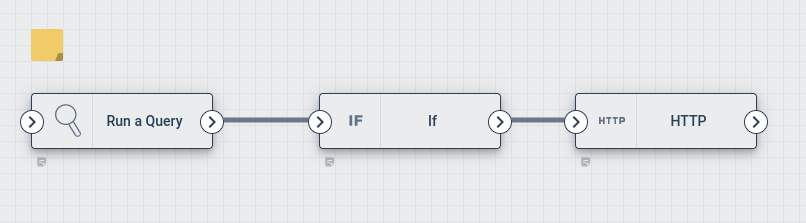
\includegraphics[width=0.6\linewidth]{images/note-minimized.png}
	\caption{A minimized note.}
	\label{fig:note-minimized}
\end{figure}

When clicked, the note expands and text can be entered, as shown in Figure \ref{fig:note-open}.

\begin{figure}
	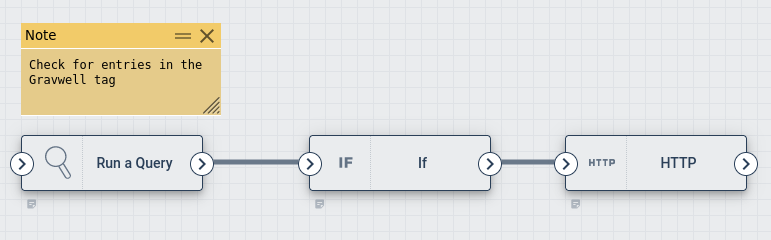
\includegraphics[width=0.6\linewidth]{images/note-open.png}
	\caption{An ``open'' note.}
	\label{fig:note-open}
\end{figure}

Clicking the ``X'' will minimize the note, leaving the start of the text visible as seen in Figure \ref{fig:note-multiple}.

\begin{figure}
	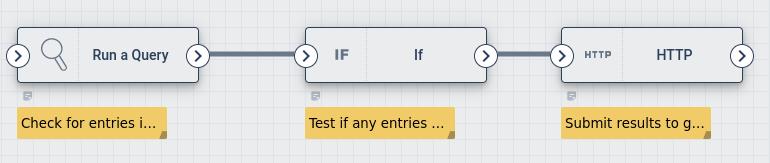
\includegraphics[width=0.6\linewidth]{images/note-multiple.png}
	\caption{Multiple minimized notes with text preview visible.}
	\label{fig:note-multiple}
\end{figure}

\clearpage
\subsection{Nodes}
\label{sec:nodes}

The following nodes are currently implemented:

\begin{itemize}
\item Email: send email messages.
\item Flow Storage Read: read items from a persistent storage.
\item Flow Storage Write: write items into a persistent storage.
\item Gravwell Notification: set Gravwell notifications.
\item HTTP: do HTTP requests.
\item If: perform logical operations.
\item Indexer Info: get information about Gravwell indexers.
\item Ingest: ingest data into Gravwell.
\item Ingester Info: get information about Gravwell ingesters.
\item JavaScript: run small snippets of Javascript code for custom operations.
\item Nest Merge: join multiple input payloads into one.
\item PDF: create PDF documents.
\item Query Log Ingest: convert search results to alert entries \& ingest.
\item Rename: rename variables in the payload.
\item Run a Query: run a Gravwell query.
\item Set Variables: inject variables into the payload.
\item Slack File: upload a file to a Slack channel.
\item Slack Message: send a message to a Slack channel.
\item Sleep: pause flow execution for a given period of time.
\item Stack Merge: join multiple input payloads into one.
\item Teams Message: send a Microsoft Teams message.
\item Text Template: format text.
\end{itemize}

The following nodes tend to be needed only in particular advanced cases:

\begin{itemize}
\item Get Table Results: get results from a search using the table renderer.
\item Get Text Results: get results from a search using the text renderer.
\end{itemize}

A selection of nodes are described in greater detail below. Documentation for every individual node is available on the Gravwell documentation website.\footnote{\href{https://docs.gravwell.io/\#!flows/flows.md}{https://docs.gravwell.io/\#!flows/flows.md}}

\subsubsection{Nest Merge Node}
The Nest Merge node can join multiple input payloads into a single output payload. It ``nests'' each input payload under a different name in the outgoing payload. Figures \ref{fig:nestmerge1} and \ref{fig:nestmerge2} show a simplified example of how this works. Two Set Variable nodes are instantiated, each injecting a variable named ``foo''; the first sets the value to \code{first value} and the other sets the value to \code{second value}. The outputs of these nodes are fed to the Nest Merge node, which has been configured with two input sockets named \code{x1} and \code{x2}. Figure \ref{fig:nestmerge2} shows how the Nest Merge node places the incoming payloads under new top-level names corresponding to the input sockets; thus the \code{foo: "first value"} output of the first Set Variable node is nested under the name \code{x1}.

\begin{figure}
	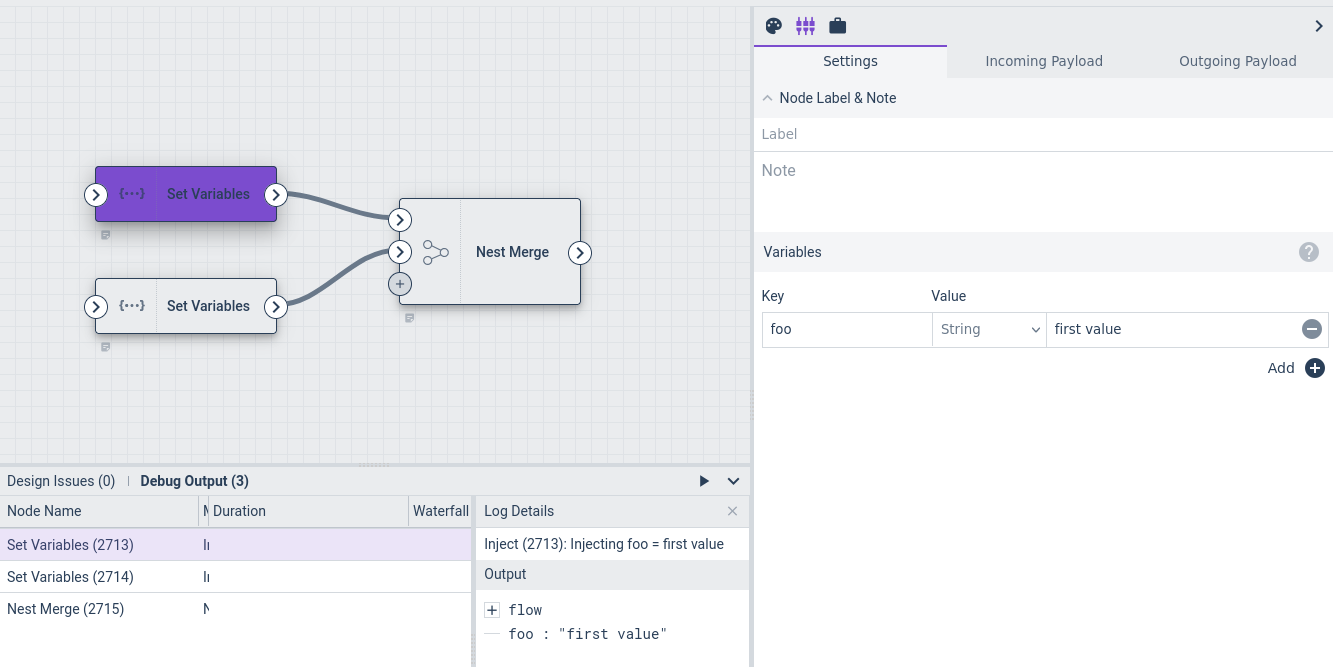
\includegraphics[width=0.85\linewidth]{images/nestmerge1.png}
	\caption{Nest merge inputs.}
	\label{fig:nestmerge1}
\end{figure}

\begin{figure}
	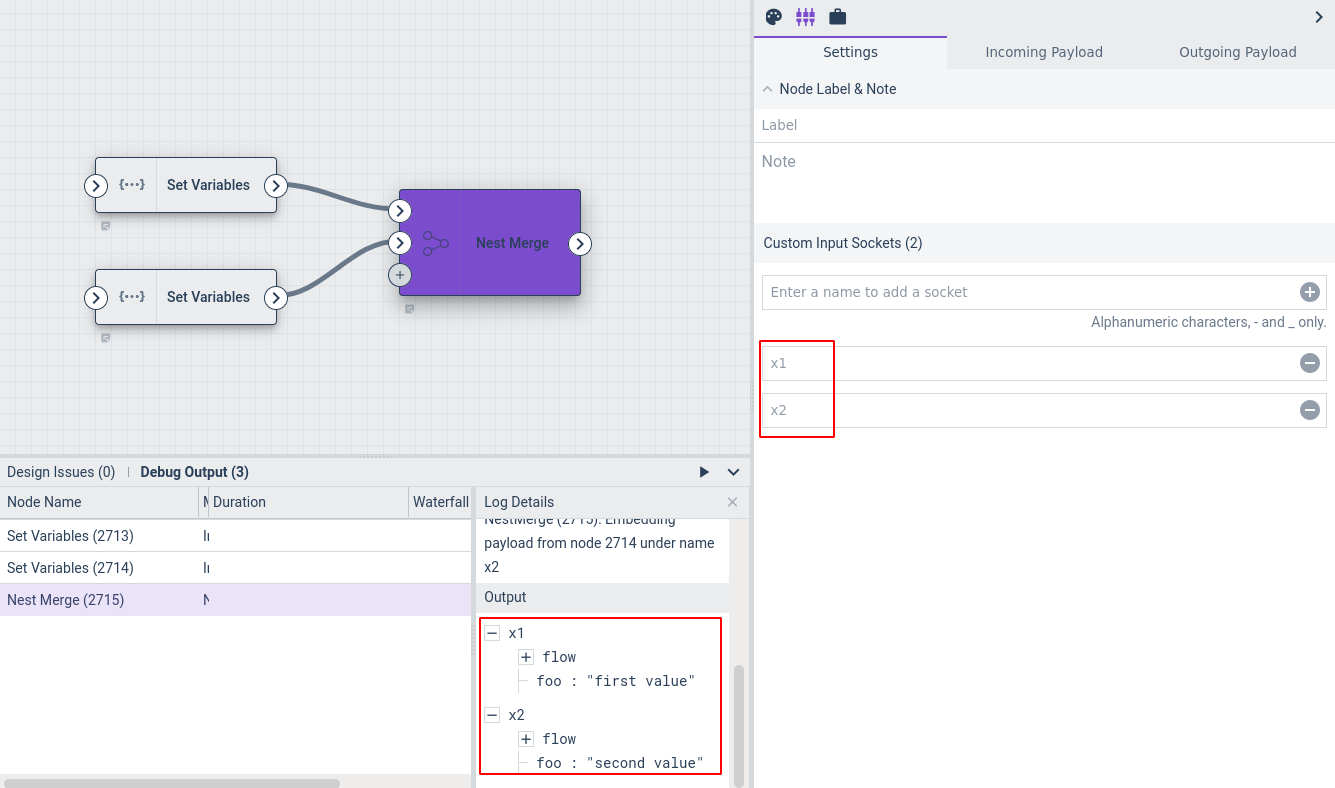
\includegraphics[width=0.85\linewidth]{images/nestmerge2.png}
	\caption{Nest merge output.}
	\label{fig:nestmerge2}
\end{figure}

\subsubsection{Stack Merge Node}
The Stack Merge node can join multiple input payloads into a single output payload. Where the Nest Merge node ``nests'' input payloads and thus always preserves the entirety of all inputs, the Stack Merge node ``overlays'' inputs. That is, it takes the first input payload, then merges in the second payload, \emph{overwriting} any variables with the same name. It repeats this process for all input payloads.

Figures \ref{fig:stackmerge1} and \ref{fig:stackmerge2} show a simplified example of how this works. Two Set Variable nodes are instantiated, each injecting a variable named ``foo''; the first sets the value to \code{first value} and the other sets the value to \code{second value}. The first node also injects a variable named ``x'' with a value of \code{y}.

The outputs of these nodes are fed to the Stack Merge node, which has been configured with two input sockets. Figure \ref{fig:stackmerge2} shows how the Stack Merge node overwrites values; thus the \code{foo: "first value"} output of the first Set Variable node is overwritten by the second node's \code{foo: "second value"} output, but the ``x'' variable is preserved since the second node does not set a variable with the same name.

\begin{figure}
	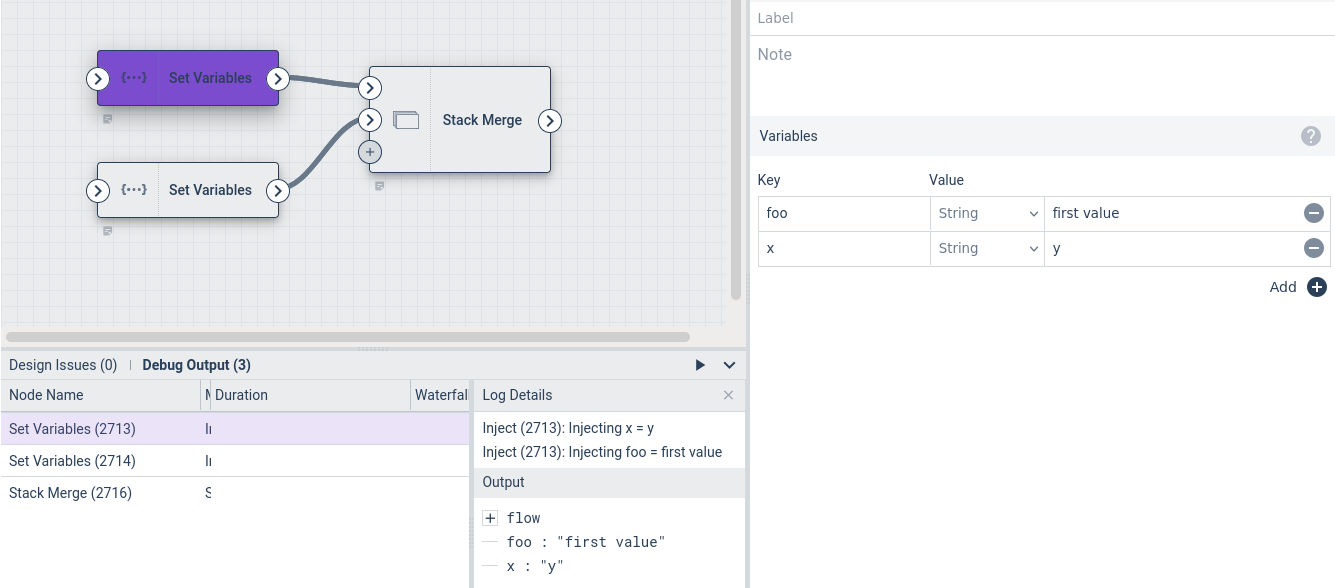
\includegraphics[width=0.85\linewidth]{images/stackmerge1.png}
	\caption{Stack merge inputs.}
	\label{fig:stackmerge1}
\end{figure}

\begin{figure}
	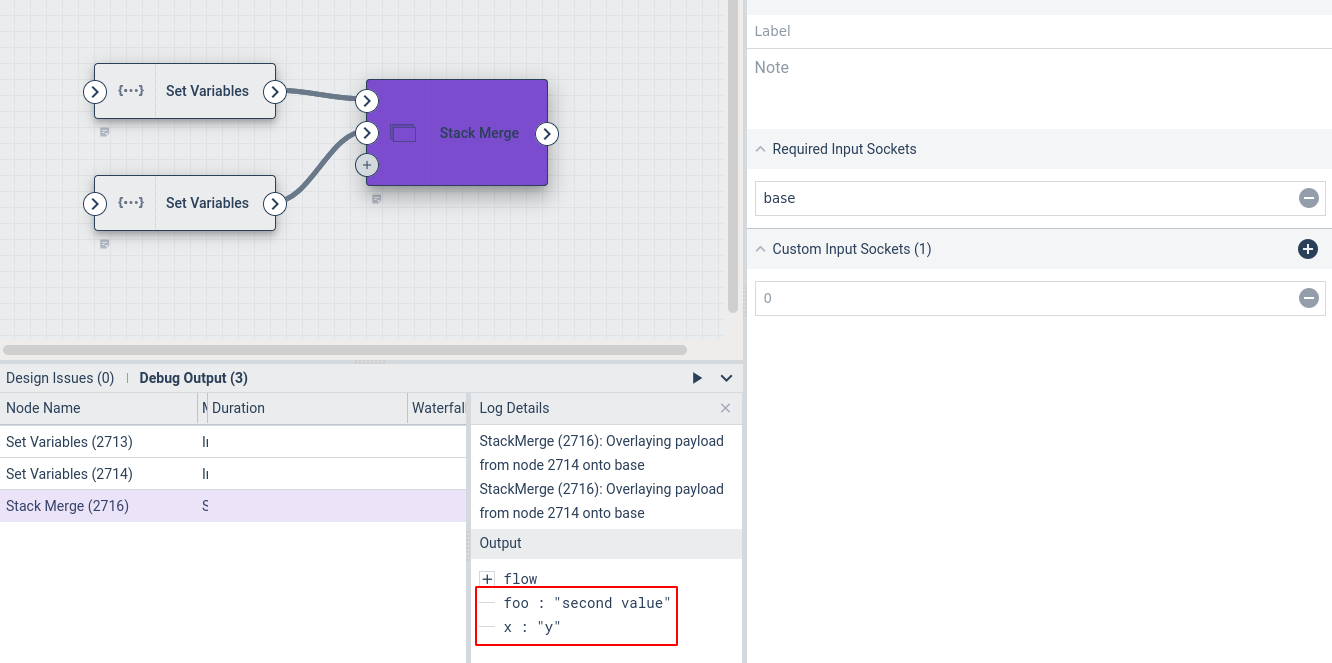
\includegraphics[width=0.85\linewidth]{images/stackmerge2.png}
	\caption{Stack merge output.}
	\label{fig:stackmerge2}
\end{figure}

\subsubsection{Email Node}
The Email node sends emails from within a flow. It can attach items from the payload. Note that the user who owns the flow \emph{must} configure an email server as described in Section \ref{sec:account-menu} for the Email node to function properly!

\begin{itemize}
\item Sender, required: This is the address which will appear in the ``From'' header of the email.
\item Recipients, required: The email will be sent to this address or addresses.
\item Subject, required: The subject line of the email.
\item Body, required: The body text of the email message. Enter a string manually, or select a variable containing suitable text. The Text Template node provides powerful tools for formatting text in the flow.
\item Attachments: An optional array of items to add as attachments on the email.
\end{itemize}

The Email node makes a best-effort attempt at determining the appropriate file type on the attachment. Naming payload items with appropriate file extensions (e.g. appending \code{.pdf} to the output name of the PDF node) helps the Email node figure out the correct type, but it can also make some deductions based on the structure of the data.

\subsubsection{JavaScript Node}
The JavaScript node can execute JavaScript code in a flow, allowing complex logic and custom operations on the payload. The configuration of a JavaScript node consists of three items:

\begin{itemize}
\item Code: the actual JavaScript code to execute.
\item Libraries: a set of libraries to load; these are key-value pairs, where the key is the name of the library (for user reference only) and the value is the content of the library.
\item Outputs: a list of variables to be output from the script (see below).
\end{itemize}

Scripts can read from and write to the payload by accessing the \code{payload} variable, e.g. \code{payload.flow.Scheduled}. Note that variables \emph{created} in the payload are only visible to downstream nodes if that variable is explicitly listed in the ``Outputs'' configuration field.

Combining the HTTP node and the JavaScript node makes it trivially easy to load JS libraries from the Internet. For instance, the flow in Figure \ref{fig:js-flow} uses the HTTP node to fetch the Moment JavaScript library\footnote{https://momentjs.com/downloads/moment-with-locales.min.js}, then the JavaScript node loads the HTTP response as a library and uses it to format a timestamp.

\begin{figure}
	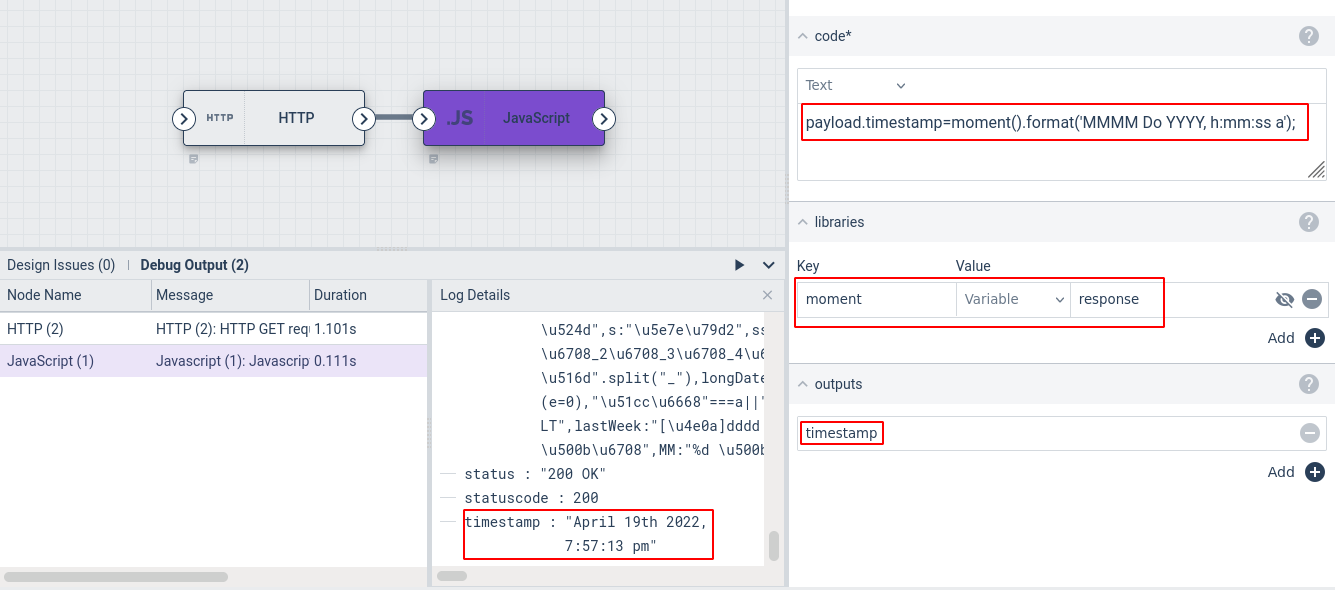
\includegraphics[width=0.85\linewidth]{images/js-flow.png}
	\caption{Loading JavaScript libraries.}
	\label{fig:js-flow}
\end{figure}

\subsubsection{PDF Node}
The PDF node formats search results and other data into an attractive PDF document, which can then be sent to recipients using the Email node, the Slack node, the HTTP node, etc.

There are many configuration options on the PDF node:

\begin{itemize}
\item Title, required: the title of the PDF.
\item Subtitle: an optional sub-title.
\item Contents, required: select one or more items from the payload to be included in the PDF. Query results will be automatically formatted.
\item Page Size: change the size of the pages in the PDF.
\item Include Flow Metadata Page: if set to true, the PDF will include a final page giving information about the execution of the flow.
\item Password: if set, the PDF will be password-protected.
\item Output Variable Name: sets the name for the output PDF in the payload.
\end{itemize}

The ``Contents'' field is perhaps the most critical. The node will attempt to format each item in this field as a section within the PDF document. It knows how to parse query results, meaning that a query using the table renderer will be inserted into the PDF as a proper table. Figure \ref{fig:pdf-contents} shows an example flow in which the outputs of several queries, plus the output of a Text Template node, are used as the Contents of a PDF. Figure \ref{fig:pdf-result} shows an example of what such a PDF may look like.

\begin{figure}
	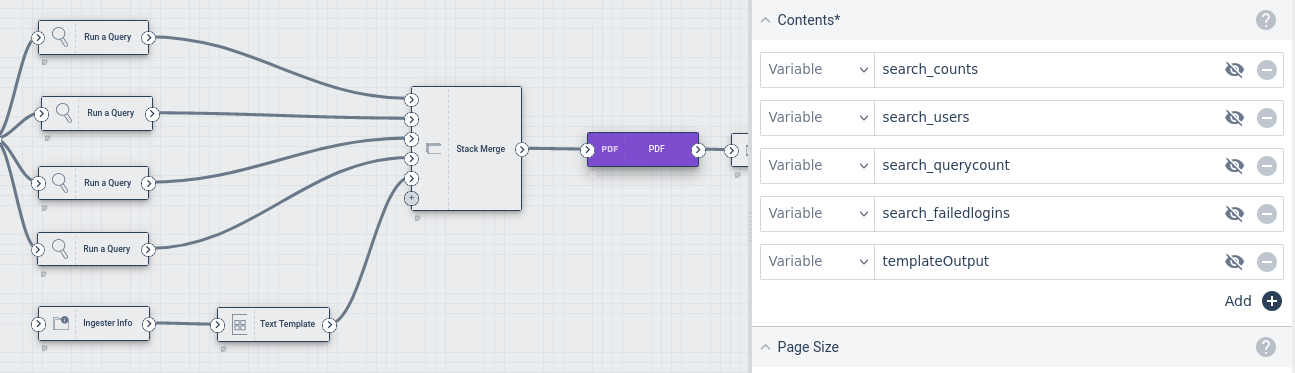
\includegraphics[width=0.95\linewidth]{images/pdf-contents.png}
	\caption{Including multiple query results in a PDF.}
	\label{fig:pdf-contents}
\end{figure}

\begin{figure}
	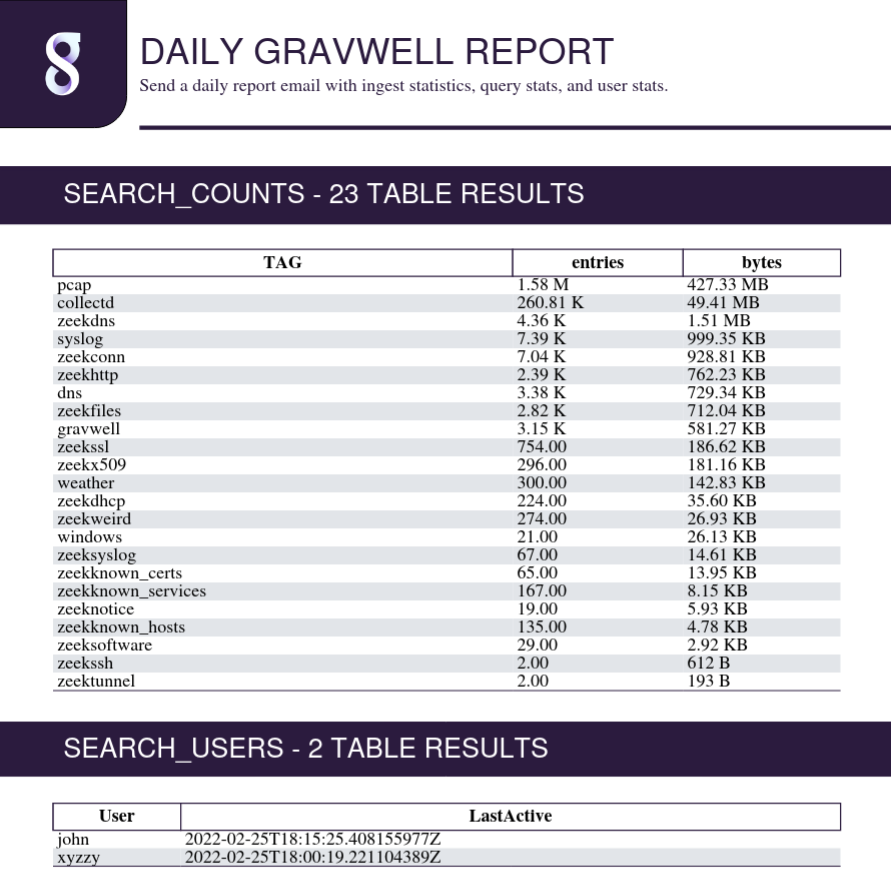
\includegraphics[width=0.85\linewidth]{images/pdf-result.png}
	\caption{Sample PDF output.}
	\label{fig:pdf-result}
\end{figure}

The ``Output Variable Name'' config option specifies the name to use for the output PDF in the payload. Using a name which ends in \code{.pdf} will help inform other nodes that the object is a PDF file, for instance when included as an attachment on the Email node.

Setting ``Include Flow Metadata Page'' to true causes the node to insert an additional page at the end of the document containing additional information about the user who executed the flow, the status of the Gravwell cluster, and the current Gravwell license. It will also insert the full query string, the timeframe, and the execution time for any queries which were packaged into the PDF.
\clearpage

\subsubsection{Slack File/Message Nodes}
Two nodes can send to Slack: Slack Message and Slack File. As the names imply, one sends a text message to a Slack channel, while the other uploads a file. Both nodes have the following configuration options:

\begin{itemize}
\item Token, required: a Slack access token\footnote{\href{https://api.slack.com/authentication/token-types}{https://api.slack.com/authentication/token-types}} for the desired server.
\item Channel, required: the channel that will receive the message, \emph{without} a preceding `\#' character.
\item Message: the message body; Markdown is supported.
\end{itemize}

The Slack Message node also has a ``Verbatim Text'' config, which is optional text to be attached to the message verbatim, without being parsed as Markdown. This is useful for showing the result of an HTTP request or other unformatted data.

The Slack File node also has a ``File to Send'' config, which is an item from the payload to be attached to the message. This works particularly well with the output of the PDF node.

Note that any user with read access to the flow will be able to extract the token, giving them the ability to write to the same Slack server. For this reason, we recommend that flows with Slack nodes should not be shared with other users.

\subsubsection{Teams Node}
The Teams node can send a message to a Microsoft Teams channel. The configuration options are:

\begin{itemize}
\item Webhook, required: an incoming webhook\footnote{\href{https://docs.microsoft.com/en-us/microsoftteams/platform/webhooks-and-connectors/what-are-webhooks-and-connectors}{https://docs.microsoft.com/en-us/microsoftteams/platform/webhooks-and-connectors/what-are-webhooks-and-connectors}} URL for Microsoft Teams.
\item Title: an optional title for the message.
\item Message, required: the body of the message to send.
\end{itemize}

Note that any user with read access to the flow will be able to extract the webhook, giving them the ability to write to the same Teams channel. For this reason, we recommend that flows with Teams nodes should not be shared with other users.

\clearpage
\subsection{Hands-On Lab: Flows}

This lab will demonstrate how to build a flow. The flow will send a notification whenever there have been failed login attempts to the Gravwell system. First, create a Gravwell webserver+indexer container:

\begin{Verbatim}[breaklines=true]
docker run -d --rm --net gravnet -p 8080:80 --name gravwell gravwell:base
\end{Verbatim}

Now log into the web GUI (\href{http://localhost:8080}{http://localhost:8080}). After that, open a new \emph{private} browser window (so the existing login cookie isn't used) and enter some invalid login credentials, e.g. username ``admin'' with password ``admin''. This will generate a login failure message which we can check using the following query:

\begin{Verbatim}[breaklines=true]
tag=gravwell syslog Message=="Authentication failure" user 
| stats count by user 
| table user count
\end{Verbatim}

\begin{figure}
	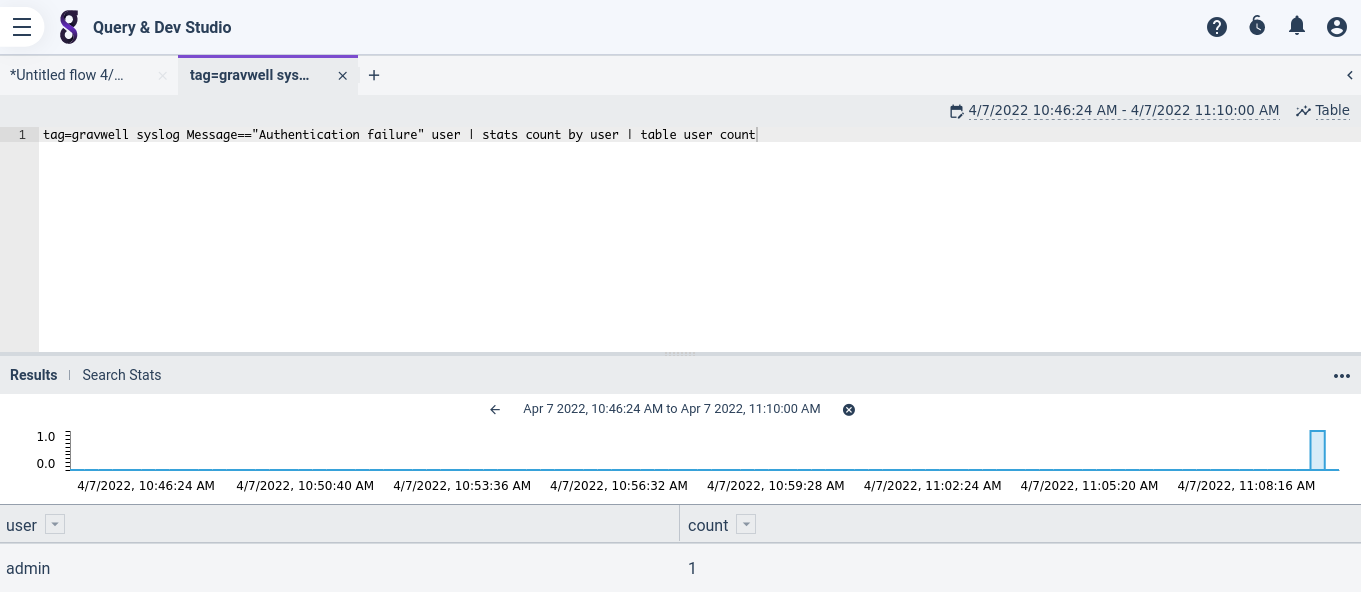
\includegraphics[width=0.85\linewidth]{images/lab-failed-logins.png}
	\caption{Query showing failed login attempts.}
	\label{fig:lab-failed-logins}
\end{figure}

We will use that query as the basis for a new flow. Select ``Flows'' from the ``Automation \& Flows'' section in the main menu, then click the ``+'' icon in the upper right to create a new flow. Drag the following nodes from the node palette out to the canvas:

\begin{itemize}
\item Run a Query
\item If
\item Gravwell Notification
\end{itemize}

Wire them up as seen in Figure \ref{fig:lab-nodes}

\begin{figure}
	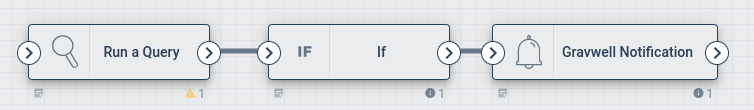
\includegraphics[width=0.7\linewidth]{images/lab-nodes.png}
	\caption{Node layout for lab.}
	\label{fig:lab-nodes}
\end{figure}

Each node now needs to be configured. Begin with the Run a Query node; click it, then paste the Gravwell query above into the ``Query String'' config field. Note how the ``Search Timeframe'' defaults to the last hour, and ``Output Variable Name'' defaults to ``search''. This means the payload output by the Run a Query node will contain an item named ``search'' with information about the query which was executed.

The If node should be configured to check \code{search.Count > 0}. This means that execution will continue if there were any results from the search.

Finally, set a message in the Gravwell Notification node's Message field, something like ``Failed logins! Go check!''.

Once all three nodes are configured, the Design Issues tab of the console should be empty. If there are issues reported, check your configuration on the associated node.

To test the flow, click the debug icon in the toolbar. You should soon see a notification appear as in Figure \ref{fig:lab-notification}.

\begin{figure}
	
\includegraphics[width=0.7\linewidth]{images/lab-notification.png}
	\caption{Example notification from flow.}
	\label{fig:lab-notification}
\end{figure}

If no notification appears, double-check that the query given above actually returns results when run over the last hour, or try generating more failed login attempts.

Once the flow is working, you can prepare the flow for deployment.  In the Run Query node's config, change the Search Timeframe dropdown from ``ISO Duration'' to ``Variable''. The value should change to the default \code{flow.Interval}. Then go to the Info \& Scheduling tab, set the schedule to ``* * * * *'' to make it run every minute, toggle the ``Disable scheduling'' slider, and hit Save. These two changes will make the flow run automatically every minute, and cause the query to run only over the last minute (this is the effect of setting the duration to \code{flow.Interval}).

Test these changes by periodically creating failed login events. You should see a notification pop up after a failed login. Delete the notification; it should not come back again until you do another failed login.

To clean up after the experiment, run:

\code{docker kill \$(docker ps -a -q)}


\section{Search Scripting and Orchestration}

Scripts provide an additional layer of power beyond scheduled
searches. A script can execute multiple searches, filter and enrich the
results, then re-ingest the resulting entries under a different tag,
send alerting emails, or do HTTP requests automatically.

Scripts can be run on a schedule, just like scheduled searches, or they
can be run manually with the command line client. This section will
first discuss how scripts are written, then delve into examples of how
they can be run and used.

A script can be scheduled in exactly the same way as a scheduled search
by simply changing the dropdown in the scheduled search creation form
from ``Search query'' to ``Anko script'' and pasting the script into the
form, as shown in Figure \ref{fig:create-soar}.

\begin{figure}
	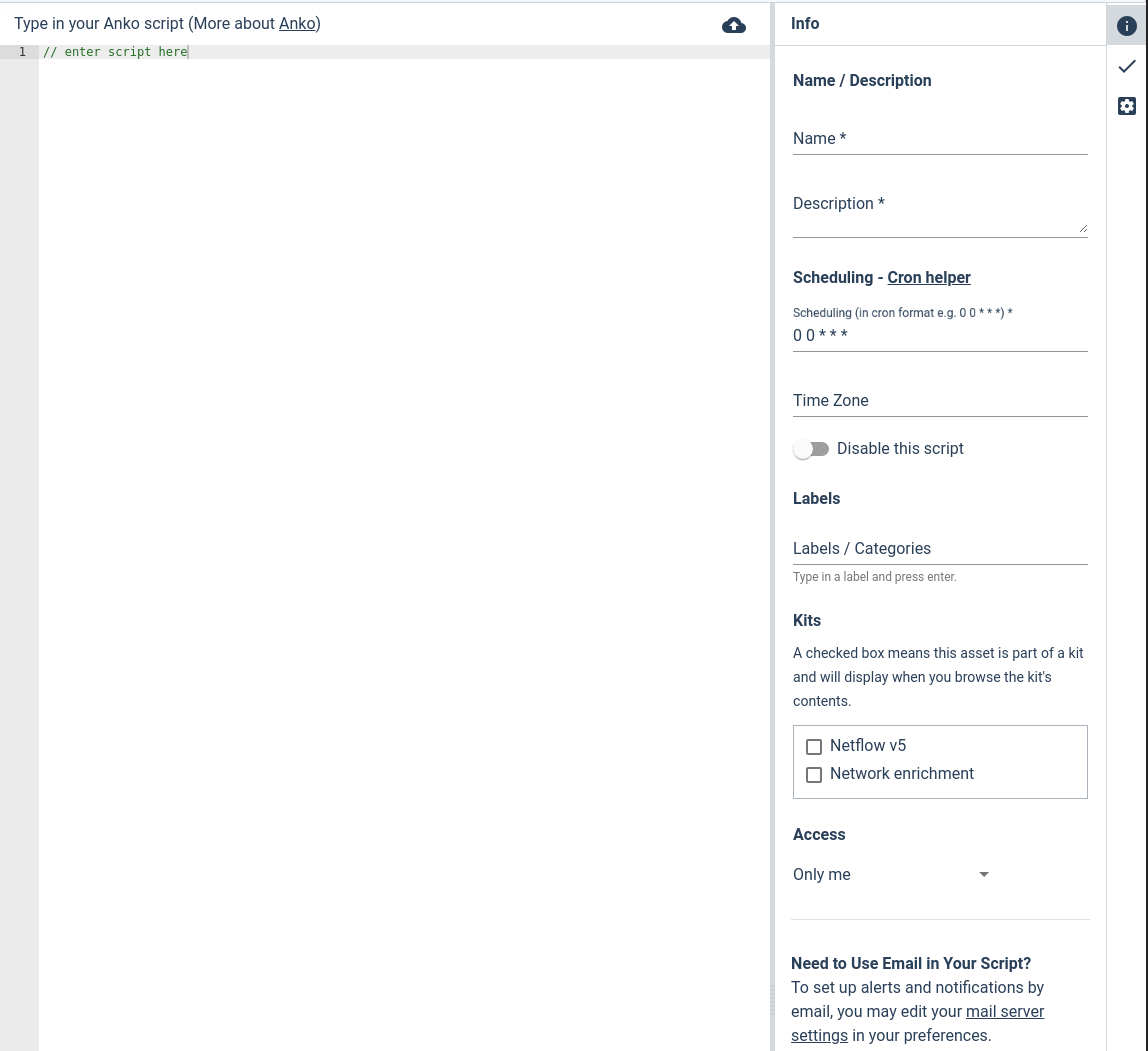
\includegraphics{images/create-soar.png}
	\caption{Creating a new scheduled script}
	\label{fig:create-soar}
\end{figure}

The rest of this section will describe what scripts look like and how
they are written.

\subsection{The Anko Scripting Language}

Gravwell scripts are written in the Anko scripting language (see
\href{http://github.com/mattn/anko}{http://github.com/mattn/anko}).
Anko is an interpreted, dynamically-typed language whose syntax
resembles Go. This section gives a brief overview of the language.

\subsubsection{Comments}

Anko comments can be prefixed with either the hash character or a pair
of slashes, or they can be wrapped in C-style comment markers:

\begin{Verbatim}[breaklines=true]
    // This is a valid Anko comment
    # This is also a valid comment
    /* This is a comment, too */
\end{Verbatim}

\subsubsection{Declaring variables}

In Anko, variables can be created and modified with the same syntax:

\begin{Verbatim}[breaklines=true]
    // This creates the variable
    x = 1
    // And this updates it
    x = x + 1
\end{Verbatim}


The `var' keyword can be used to indicate that a \emph{new} variable
\emph{must} be allocated at the current scope:

\begin{Verbatim}[breaklines=true]
    // Declare a variable
    var x = 1

    if true {
        // Declare a new variable at the inside scope
        var x = 2
    }
    println(x)    // prints “1”
\end{Verbatim}

If the `var' keyword was not used, the \code{println} call would have
printed `2'.

\subsubsection{Slices}

Anko implements slices (arrays) in a similar way to Go, but with more implicit
operations allowed:

\begin{Verbatim}[breaklines=true]
    a = [1, 2, 3]
    a += 4        // append
    println(a)    // prints [1 2 3 4]
    println(a[1])    // prints 2
\end{Verbatim}

Anko's default slice type is \code{[]interface\{\}}, which means a
slice can contain many different types. Note that slices are
``expanded'' when appended:

\begin{Verbatim}[breaklines=true]
    a = [1, 2.2, “foo”]
    a += [3, 4]
    a += [ [5, 6] ]
    println(a)    // prints [1 2.2 foo 3 4 [5 6]]
\end{Verbatim}


\subsubsection{Maps}

Anko maps are maps of \code{interface\{\}} to \code{interface\{\}}, meaning a
given map can mix key and value types:

\begin{Verbatim}[breaklines=true]
    m = { “foo”: 2 }    // initializes a map with a single entry, “foo” -> 2
    m[3] = 7        // map key 3 to value 7
    println(m[3])    // prints “7”
    println(m[“foo”]) // prints “2”
\end{Verbatim}


\subsubsection{If-Else Statements}

If-ElseIf-Else statements work exactly the same in Anko as in Go:

\begin{Verbatim}[breaklines=true]
    if x > 10 || y {
        count1++
    } else if x == 3 && !y {
        count2++
    } else {
        count3++
    }
\end{Verbatim}


\subsubsection{Switch Statements}

Anko provides switch statements similar to Go. Note that there is no
``fallthrough'' keyword.

\begin{Verbatim}[breaklines=true]
    switch val {
    case “foo”:
        count1++
    case 3:
        count2++
    default:
        notfound++
    }
\end{Verbatim}


\subsubsection{For Loops}

Anko supports traditional for loops:

\begin{Verbatim}[breaklines=true]
    for i = 0; i < 10; i++ {
      println(i)
    }
\end{Verbatim}

It also can also iterate over the contents of a slice:

\begin{Verbatim}[breaklines=true]
    a = ["foo", 3, 8.3]
    for i in a {
      println(i) // will print “foo”, 3, 8.3
    }
\end{Verbatim}

The `range' built-in function is convenient for iteration:

\begin{Verbatim}[breaklines=true]
    // this will print 0 through 9
    for i in range(0, 10) {
      println(i)
    }
    
    // this will print 0, 2, 4, 6, 8
    for i in range(0, 10, 2) {
      println(i)
    }
\end{Verbatim}

\subsubsection{Function Declaration}

Anko functions resemble Go functions, but they do not declare any
return types. Arguments are passed by value, not by reference:

\begin{Verbatim}[breaklines=true]
    func foo(x) {
      return x++
    }
    
    var a = 1
    foo(a)
    println(a)    // prints "1"
    a = foo(a)
    println(a)    // prints "2"
\end{Verbatim}

\subsection{Available Libraries}

A selection of Go libraries have some functionality exported to Anko for
use in scripts. Check the Gravwell online documentation for a full list.
Some examples are:

\begin{itemize}
\item ``bytes''
\item ``encoding/json''
\item ``errors''
\item ``math''
\item ``math/big''
\item ``math/rand''
\item ``net/url''
\item ``path''
\item ``path/filepath''
\item ``regexp''
\item ``sort''
\item ``strings''
\item ``time''
\item ``io''
\item ``flag''
\item ``io/ioutil''
\item ``encoding/csv''
\item ``crypto/md5''
\item ``crypto/sha1''
\item ``crypto/sha256''
\item ``crypto/sha512''
\item ``net''
\item ``net/http''
\item ``github.com/ziutek/telnet''
\item ``google/uuid'' (github.com/google/uuid)
\end{itemize}

Libraries must be imported using the import function before use:

\begin{Verbatim}[breaklines=true]
    var md5 = import(“crypto/md5”)
    fooSum = md5.Sum(“foo”)
\end{Verbatim}

\subsection{Gravwell Anko Functions}

Gravwell has extended the Anko language with additional functions
specifically suited to writing orchestration scripts. This section
describes those functions. The functions are listed below in the format
\code{functionName(\textless{}functionArgs\textgreater{}) \textless{}returnValues\textgreater{}}.
Functions which return more than one argument have the return values wrapped in parentheses.

\subsubsection{Resources and persistent data functions}

``Persistent maps'' are a convenience offered for scheduled searches.
Values set in a persistent map will be available for reading in
subsequent runs of the scheduled search. If the named persistent map
does not exist, it will be created. Persistent maps do nothing when the
script is run at the Gravwell CLI.

\begin{itemize}
\tightlist
\item
  \code{getResource(name) ([]byte, error) } - returns the contents of the specified resource
  as a slice of bytes, while the error is any error encountered while fetching the resource.
\item
  \code{setResource(name, value) error} - creates (if necessary) and updates
  a resource named name with the contents of value, returning an error
  if one arises.
\item
  \code{setPersistentMap(mapname, key, value)} - stores a key-value pair
  in a map which will persist between executions of a scheduled script.
\item
  \code{getPersistentMap(mapname, key) value} - returns the value
  associated with the given key from the named persistent map.
\item
  \code{delPersistentMap(mapname, key)} - deletes the specified key/value
  pair from the given map.
\end{itemize}

\subsubsection{Search entry manipulation functions}

These functions get, set, and delete enumerated values on a single
entry (as returned by the \code{getEntries} function described later)

\begin{itemize}
\tightlist
\item
  \code{setEntryEnum(ent, key, value)} - sets an enumerated value on the
  specified entry.
\item
  \code{getEntryEnum(ent, key) (value, error)} - reads an enumerated value
  from the specified entry.
\item
  \code{delEntryEnum(ent, key)} - deletes the specified enumerated value
  from the given entry.
\end{itemize}

\subsubsection{General utility functions}

\begin{itemize}
\tightlist
\item
  \code{len(val) int} - returns the length of val, which can be a string,
  slice, etc.
\item
  \code{toIP(string) IP} - converts string to an IP, suitable for comparing
  against IPs generated by e.g. the packet module.
\item
  \code{toMAC(string) MAC} - converts string to a MAC address.
\item
  \code{toString(val) string} - converts val to a string.
\item
  \code{toInt(val) int64} - converts val to an integer if possible.
  Returns 0 if no conversion is possible.
\item
  \code{toFloat(val) float64} - converts val to a floating point number
  if possible. Returns 0.0 if no conversion is possible.
\item
  \code{toBool(val) bool} - attempts to convert val to a boolean.
  Returns false if no conversion is possible. Non-zero numbers and the
  strings ``y'', ``yes'', and ``true'' will return true.
\item
  \code{typeOf(val) type} - returns the type of val as a string, e.g.
  ``string'', ``bool''.
\end{itemize}

\subsubsection{Search management functions}

Due to the way Gravwell's search system works, some of the functions in
this section return Search structs (written as \code{``search''} in the
parameters) while others return search IDs (written as
\code{``searchID''} in the parameters). Each Search struct contains a
search ID, which can be accessed as \code{search.ID}.

Search structs are used to actively read entries from a search, while
search IDs tend to refer to inactive searches to which we may attach or
otherwise manage.

\begin{itemize}
\tightlist
\item
  \code{startBackgroundSearch(query, start, end) (search, err)} - creates
  a backgrounded search with the given query string, executed over the
  time range specified by 'start' and 'end'. The return value is a
  Search struct. These time values should be specified using the time
  library; see the examples for a demonstration.
\item
  \code{startSearch(query, start, end) (search, err)} - acts exactly like
  \code{startBackgroundSearch}, but does not background the search.
\item
  \code{detachSearch(search)} - detaches the given search (a Search
  struct). This will allow non-backgrounded searches to be automatically
  cleaned up and should be called whenever you're done with a search.
\item
  \code{attachSearch(searchID) (search, error)} - attaches to the search
  with the given ID and returns a Search struct which can be used to
  read entries etc.
\item
  \code{getSearchStatus(searchID) (string, error)} - returns the status of
  the specified search, which can be ``ACTIVE'', ``ATTACHED'', ``DORMANT'', ``SAVED'', ``SAVING'', or ``UNKNOWN''.
\item
  \code{getAvailableEntryCount(search) (uint64, bool, error)} - returns
  the number of entries that can be read from the given search, a
  boolean specifying if the search is complete, and an error if anything
  went wrong.
\item
  \code{getEntries(search, start, end) ([]SearchEntry, error)} - pulls
  the specified entries from the given search. The bounds for start and
  end can be found with the \code{getAvailableEntryCount} function.
\item
  \code{isSearchFinished(search) (bool, error)} - returns true if the
  given search is complete
\item
  \code{executeSearch(query, start, end) ({[}{]}SearchEntry, error)} -
  starts a search, waits for it to complete, retrieves up to ten
  thousand entries, \emph{detaches} from search and returns the entries.
\item
  \code{deleteSearch(searchID) error} - deletes the search with the
  specified ID
\item
  \code{backgroundSearch(searchID) error} - sends the specified search to
  the background; this is useful for ``keeping'' a search for later manual
  inspection.
\item
  \code{downloadSearch(searchID, format, start, end) ({[}{]}byte,
  error)} - downloads the given search as if a user had clicked the
  'Download' button in the web UI. \code{format} should be a string containing
  either ``json'', ``csv'', ``text'', ``pcap'', or ``lookupdata'' as appropriate.
  \code{start} and \code{end} are time values.
\item
  \code{getDownloadHandle(searchID, format, start, end) (io.Reader,
  error)} - returns a streaming handle to the results of the given
  search as if the user had clicked the 'Download' button in the web UI.
  The handle returned is suitable for use with the HTTP library
  functions shown later in this document.
\end{itemize}

\subsubsection{Search Data Type}

When executing a search via the \code{startSearch} or
\code{startBackgroundSearch} functions the \emph{search} data type is
returned. The search data type contains the following members:

\begin{itemize}
\tightlist
\item
  \code{ID} - A string containing the search ID. Use this member for other
  functions like \code{getSearchStatus} and \code{attachSearch}.
\item
  \code{RenderMod} - A string indicating the renderer attached to the
  search. It may be something like raw, text, table, chart, or fdg.
\item
  \code{SearchString} - A string containing the search string passed in
  during the request
\item
  \code{SearchStart} - A string containing the start timestamp for the
  search
\item
  \code{SearchEnd} - A string containing the end timestamp for the search
\item
  \code{Background} - A boolean indicating whether the search was started as
  a background search
\item
  \code{Name} - An optional string with a search name.
\end{itemize}

\subsubsection{Transmitting alerts or search results}

The scripting system provides several methods for transmitting script
results to external systems.

The following functions provide basic HTTP functionality:

\begin{itemize}
\tightlist
\item
  \code{httpGet(url) (string, error)} - performs an HTTP GET request on the
  given URL, returning the response body as a string.
\item
  \code{httpPost(url, contentType, data) (response, error)} - performs an
  HTTP POST request to the given URL with the specified content type
  (e.g. ``application/json'') and the given data as the POST body.
\end{itemize}

More elaborate HTTP operations are possible with the ``net/http''
library. See the package documentation in
the online anko
documentation\footnote{https://docs.gravwell.io/\#!scripting/scriptingsearch.md} for a description of what is available.

If the user has configured their personal email settings within
Gravwell, the email function is a very simple way to send an email:

\begin{itemize}
\tightlist
\item
  \code{email(from, to, subject, message) error} - sends an email via SMTP.
  The from field is simply a string, while to should be a slice of
  strings containing email addresses. The subject and message fields are
  also strings which should contain the subject line and body of the
  email.
\end{itemize}

\subsubsection{Creating and ingesting entries}

It is possible to ingest new entries into the indexers from within a
script using the following functions:

\begin{itemize}
\tightlist
\item
  \code{newEntry(time, data) Entry} - returns a new entry with the
  given timestamp (a \code{time.Time}, as from \code{time.Now()}) and
  \code{data} (frequently a string).
\item
  \code{ingestEntries(entries, tag) error} - ingests the given slice of
  entries (\code{[]Entry}) with the specified tag string.
\end{itemize}

The entries returned by the \code{getEntries} function can be modified if
desired and re-ingested via \code{ingestEntries}, or new entries can be created
from scratch. For example, to re-ingest some entries from a previous search
into the tag ``newtag'':

\begin{Verbatim}[breaklines=true]
    # Get the first 100 entries from the search
    ents, _ = getEntries(mySearch, 0, 100)
    ingestEntries(ents, "newtag")
\end{Verbatim}

To ingest new entries based on some other condition:

\begin{Verbatim}[breaklines=true]
    if condition == true {
        ents = make([]Entry)
        ents += newEntry(time.Now(), "Script condition triggered")
        ingestEntries(ents, "results")
    }
\end{Verbatim}

\subsection{Example Scripts}

This script creates a backgrounded search that finds which IPs have
communicated with Cloudflare's 1.1.1.1 DNS service over the last day. If
no results are found, the search is deleted, but if there are results
the search will remain for later perusal by the user in the `Persistent
Searches' screen of the GUI.


%%%%%%%%%%%%%%%%%%%%%%%%%%%%%%
% TODO: make sure this actually works
%%%%%%%%%%%%%%%%%%%%%%%%%%%%%%

\begin{Verbatim}[breaklines=true]
# Import the time library
var time = import("time")
# Define start and end times for the search
start = time.Now().Add(-24 * time.Hour)
end = time.Now()
# Launch the search
s, err = startSearch("tag=netflow netflow Dst==1.1.1.1 Src | unique Src | table Src", start, end)
if err != nil {
    return err
}
# Wait until the search is finished
for {
    f, err = isSearchFinished(s)
    if err != nil {
        return err
    }
    if f {
        break
    }
    time.Sleep(1 * time.Second)
}
# Find out how many entries were returned
c, _, err = getAvailableEntryCount(s)
if err != nil {
    return err
}
# If no entries returned, delete the search
# Otherwise, background it
if c == 0 {
    deleteSearch(s.ID)
} else {
    err = backgroundSearch(s.ID)
    if err != nil {
        return err
    }
}
# Always detach from the search at the end of execution
detachSearch(s)
\end{Verbatim}


%%%%%%%%%%%%%%%%%%%%%%%%%%%%%%
% TODO: update for the GUI
%%%%%%%%%%%%%%%%%%%%%%%%%%%%%%
\subsection{Developing \& Testing Scripts}

Because the same script can be executed as either a scheduled search or
manually with the CLI client, scripts are usually tested/developed using
the CLI client and then copied into a scheduled search later. Scripts
run with the CLI client can display printed output, which is ignored
when run on a schedule; this is particularly useful when debugging a
script.

A script can be executed manually from the client in the following
way:

\begin{Verbatim}[breaklines=true]
$ gravwell -s <server> script
script file path> /path/to/script.ank
\end{Verbatim}

A convenient way to run a script repeatedly is to use the ``watch''
modifier. The client will execute the script, then prompt to re-run. If
the script file is modified between runs, the next execution will use
the updated script. Here, a script that hashes a string with MD5 is
modified to hash using SHA1:

\begin{Verbatim}[breaklines=true]
$ gravwell -s <server> watch script
script file path>  /tmp/hash.ank
[172 189 24 219 76 194 248 92 237 239 101 79 204 196 164 216]
Hit [enter] to re-run, or [q][enter] to cancel

[11 238 199 181 234 63 15 219 201 93 13 212 127 60 91 194 117 218 138 51]
Hit [enter] to re-run, or [q][enter] to cancel
\end{Verbatim}


%%%%%%%%%%%%%%%%%%%%%%%%%%%%%%
% TODO: update for the GUI
%%%%%%%%%%%%%%%%%%%%%%%%%%%%%%
\subsection{Hands-on Lab: Scripting}

This lab will demonstrate how to send email alerts from a script. This
lab will test the script using the Gravwell CLI client, then schedule it
for automated execution.

The script will operate on Netflow records and send an alert whenever
traffic is seen originating from the 7.0.0.0/8 subnet, which in this
example stands in for a ``known bad'' subnet or subnets. In an actual
deployment, one might keep a list of known-bad subnets in a resource
lookup table (which can be automatically updated via another script!)
and compare flow records against that lookup table instead, but for
simplicity we will use a single hard-coded subnet.

First, launch a Gravwell webserver+indexer container:

\begin{Verbatim}[breaklines=true]
docker run --rm --net gravnet -p 8080:80 -d --name gravwell gravwell:base
\end{Verbatim}

Log in, go to the Account
settings page and select the Email Server tab, then populate your email
server configuration and test it (Figure \ref{fig:lab-emailsettings}).

\begin{figure}
	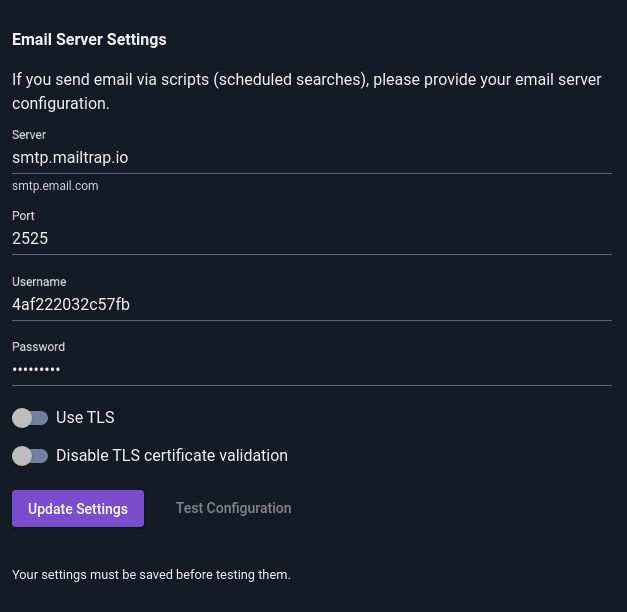
\includegraphics{images/lab-emailsettings.png}
	\caption{Configuring email server}
	\label{fig:lab-emailsettings}
\end{figure}

Next, start the ingester container running the Netflow ingester:

\begin{Verbatim}[breaklines=true]
docker run --rm -d --net gravnet --name ingesters \
-e GRAVWELL_CLEARTEXT_TARGETS=gravwell:4023 gravwell:ingesters \
/opt/gravwell/bin/gravwell_netflow_capture
\end{Verbatim}

The Netflow ingester is pre-configured to listen on port 2055 for
incoming Netflow v5 records.

Now, we use another Docker container to generate Netflow records and
send them to the ingester:

\begin{Verbatim}[breaklines=true]
docker run -it --net gravnet --rm \
networkstatic/nflow-generator -t ingesters -p 2055
\end{Verbatim}

The Netflow generator will run indefinitely, generating flow records,
until killed. Let it run at least until the following query shows at
least one result:

\begin{Verbatim}[breaklines=true]
tag=netflow netflow Src | subnet Src /8 as sub | ip sub == 7.0.0.0 | table
\end{Verbatim}

This query will form the basis of our script. It extracts the source IP
address from the Netflow records, converts that to a /8 subnet and
stores the result in an enumerated value named ``sub'', then compares
``sub'' to 7.0.0.0.

Open the file named \code{email-netflow.ank}  on the host system and paste
the following into it (or use the version in the training package):

\begin{Verbatim}[breaklines=true]
var time = import("time")
# SET THESE VARIABLES
from = "MY.ADDRESS@EXAMPLE.COM"
to = [ "RECIPIENT@EXAMPLE.COM" ]
my_name = "HANK"
# Do the search over the last day
end = time.Now()
start = end.Add(-24 * time.Hour)
query = `tag=netflow netflow Src | subnet Src /8 as sub | ip sub == 7.0.0.0 | table`
s, err = startSearch(query, start, end)
if err != nil {
        return err
}
# Wait for the search to complete
for {
        f, err = isSearchFinished(s)
        if err != nil {
                return err
        }
        if f {
                break
        }
        time.Sleep(1 * time.Second)
}
# Figure out how many results there were
c, _, err = getAvailableEntryCount(s)
if err != nil {
        return err
}
# clean up the search, we only care about how many entries there were
detachSearch(s)

# If there was more than 0 entries, send an email
if c > 0 {
        summary = "There were " + c + " flows originating from the banned subnet!"
        email(from, to, my_name + " alert!", summary)
}
\end{Verbatim}

Modify the \code{`from'}, \code{`to'}, and \code{`my\_name'} variables at the
top of the script; `from' should be your email address, `to' is a list
of email recipients (this should probably be your email address again),
and `my\_name' is your own name.

Now copy the file to the Gravwell container and run a shell:

\begin{Verbatim}[breaklines=true]
docker cp email-netflow.ank gravwell:/tmp/
docker exec -it gravwell /bin/sh
\end{Verbatim}

Within that shell, run the Gravwell CLI client and execute the script:

\begin{Verbatim}[breaklines=true]
$ gravwell -insecure-no-https script
script file path>  /tmp/email-netflow.ank
\end{Verbatim}

If all goes well, an email alert should arrive soon!

The script can be trivially run on a schedule by simply pasting it into
the New Scheduled Search dialog, as shown in Figure \ref{fig:lab-create-script}.

\begin{figure}
	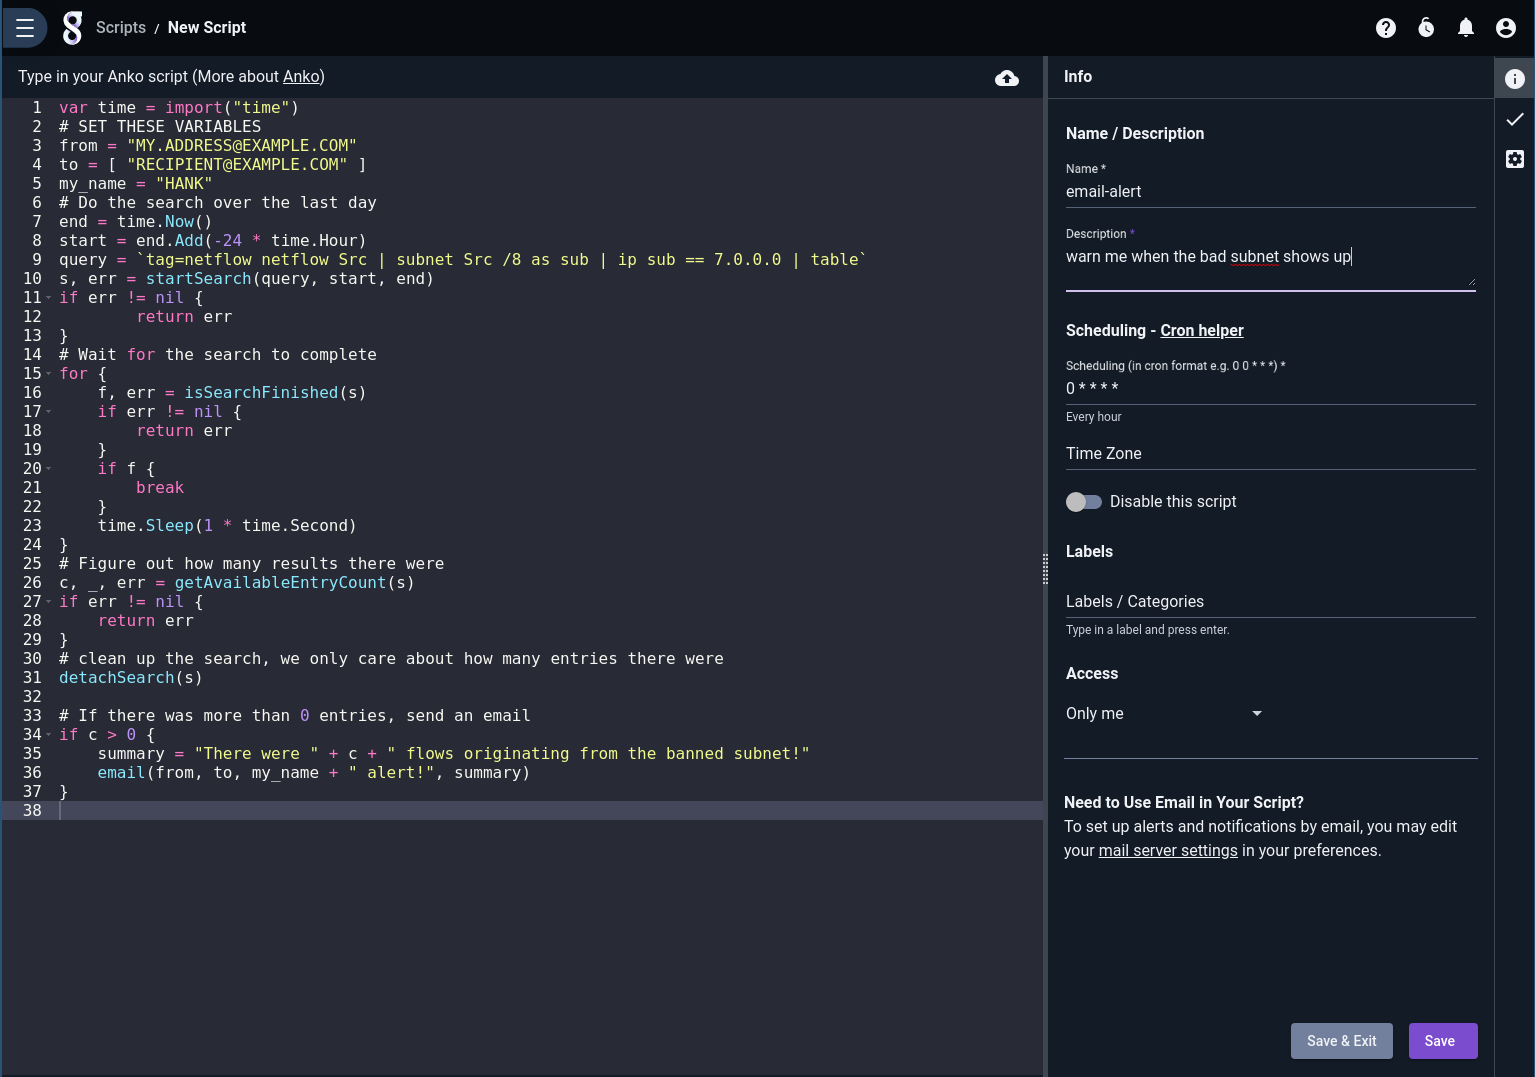
\includegraphics{images/lab-create-script.png}
	\caption{Creating scheduled script}
	\label{fig:lab-create-script}
\end{figure}

Note that this will send an email every minute, so either delete the
scheduled script once it's been verified to work, or shut down the
entire experiment when satisfied:

\code{docker kill \$(docker ps -a -q)}
